\documentclass[logo,magister]{tesis-postgrado}

% % Declaración para colocar código Java
%\usepackage{listings}
%\usepackage{color}
%
%\definecolor{dkgreen}{rgb}{0,0.6,0}
%\definecolor{gray}{rgb}{0.5,0.5,0.5}
%\definecolor{mauve}{rgb}{0.58,0,0.82}
%
%\lstset{frame=tb,
%  captionpos=b, 
%  language=Java,
%  numbers=left,
%  aboveskip=3mm,

%  belowskip=3mm,
%  showstringspaces=false,
%  columns=flexible,
%  basicstyle={\small\ttfamily},
%  %numbers=none,
%  numberstyle=\tiny\color{gray},
%  keywordstyle=\color{blue},
%  commentstyle=\color{dkgreen},
%  stringstyle=\color{mauve},
%  breaklines=true,
%  breakatwhitespace=true,
%  tabsize=3
%}

\renewcommand{\lstlistingname}{C\'ODIGO}

% % Pa usar quotes
\usepackage{csquotes}
\usepackage{rotating}


\keywords{XML; Key Implication}

\begin{document}
\baselineskip 23pt
% ----------------------------------------------------------
\thispagestyle{empty}
\titulo{Modelo de Representación y Construcción de Sistemas de Recomendación para Interacciones de la Web 2.0}

\autor{Rodrigo de Jesús Vásquez Fernández}

\fecha{Lunes}{15}{Enero}{2013} %Del Examen de Grado

\profesorguia{Dr.\ Edmundo Pablo Leiva Lobos}

\ciudad{Santiago}
\pais{Chile}
\makecubierta
\makecopyright
% ----------------------------------------------------------
\frontmatter

\begin{gracias}

El término de este trabajo representa el fin de sin duda la etapa más enriquecedora que he tenido en mi vida. Fueron 8 años dentro de una de las universidades más prestigiosas de nuestro país, donde he adquirido una formación completa desde lo técnico hasta lo valórico.

Agradezco de todo corazón a mis padres Jacqueline y Rafael por no dejar que me faltará nada durante mi formación, gracias a su esfuerzo he podido cumplir mi sueño de ser profesional. A mi hermano Cristóbal por ser mi amigo y estar siempre dispuesto a acompañarme y escucharme. A mis primos Marco y Ariel por estar siempre presentes cuando necesite ayuda. A mis tías Odette, Teresa y abuelo Jorge por estar siempre preocupados por mí. A mi ahijado Agustín por ser el mejor ahijado que existe.

A María Isabel por su amor incondicional y apoyo, gracias por apoyarme en todas mis decisiones a pesar de que algunas fueron erróneas, te amo.

A Edmundo, por ser más un amigo que un profesor guía, siempre supo aconsejarme para mitigar mi ansiedad cuando perdía el rumbo, nunca olvidaré todas las discusiones que tuvimos por mi trabajo de tesis que sin duda llegó a un excelente resultado, gracias por su formación. A Benito Contreras por enseñarme a programar en Java de manera profesional, y aconsejarme en los momentos difíciles de mi tesis. A los profesores que he tenido durante mi formación por entregarme las herramientas para desarrollar este trabajo y a los funcionarios del departamento por su disposición a resolver cualquier duda.

A mis compañeros de carrera con los que estudie y trabaje, en especial a mis amigos Sebastián, Héctor y Fabián. A mis compañeros del equipo \textit{Social-Tagging} por las reuniones donde compartimos las inquietudes sobre nuestros trabajos, Andy, Salvador, Michael, Felipe B., Felipe Q., Felipe G., Álvaro, Francisco, Fabián, Carlos, Daniel y de manera especial a Alonso por sus consejos en los momentos difíciles.

Finalmente quiero dar gracias a Dios por ser mi luz y guía en este camino.


\end{gracias}
% % AGREGADO PARA IMPRIMIR EN DOBLE CARA
\newpage\null\thispagestyle{empty}\newpage
\dedicatoria{
	Para Rubén, Flor, Tía Tita, familia y amigos
}
% % AGREGADO PARA IMPRIMIR EN DOBLE CARA
\newpage\null\thispagestyle{empty}\newpage
\resumenCastellano{
El procesamiento de transacciones de lecturas en motores de búsqueda demanda el uso eficiente de recursos de \textit{hardware} para hacer frente a altas y dinámicas cargas de trabajo por parte de los usuarios. Estos sistemas son generalmente desplegados en grupos de máquinas con múltiples procesadores cada una, de modo que puedan responder múltiples consultas simultáneamente. A medida que la Web crece, los motores de búsqueda toman mayor importancia en la búsqueda de información dentro de grandes cantidades de datos.

En el presente trabajo se abordan diferentes estrategias de procesamiento y planificación de transacciones de lectura, así como también técnicas de asignación de recursos para resolverlas, enfocadas principalmente en (1) el acceso a grandes índices invertidos para obtener el conjunto de los mejores $K$ documentos para una consulta utilizando el algoritmo Wand, y (2) el uso de predictores de eficiencia para transacciones de lectura con el objetivo de reducir el tiempo de procesar lotes de consultas.

Los resultados obtenidos muestran que se puede reducir el tiempo de procesamiento de grandes conjuntos de consultas utilizando métodos que predigan el costo en tiempo de estas y que algunos métodos de aprendizaje pueden llegar a ser dependiente de los datos. Además se obtiene que en el contexto de un motor de búsqueda, las técnicas de planificación disponibles en el estado del arte son muy dependientes de la precisión del predictor, por lo cual se propone un enfoque de procesamiento de consultas basado en unidades de trabajo con el que se obtienen mejoras significativas en los tiempos totales de procesamiento. 


\vspace*{0.5cm}
\KeywordsES{recuperación de información, motores de búsqueda, Wand}.
}

\newpage

\resumenIngles{
Processing queries in Web search engines demands the efficient use of hardware resources to cope with high and dynamics workload of the users traffic. These systems are usually deployed on dedicated clusters of servers with multiprocessors each one, so that they can respond multi-queries simultaneously. As the Web becomes bigger, search engines are becoming increasingly important to find information in large amounts of data. 

This work discusses different query processing and scheduling strategies, also it studies resources allocation techniques to resolve them, focused mainly on (1) access to large inverted index data structure to obtain the top-K most pertinent results for any query using Wand algorithm, and (2) the use of different query efficiency predictors in order to process batches of queries.
 
The results show that query efficiency predictors can lead to reduce the processing time of large query batches and them also show that some query predictors may become data dependents. This work also shows that, in the context of search engine, state of the art algorithms for query scheduling are very dependents of the predictor accuracy, whereby this work presents a query processing technique based on work units which obtains significant improvements in total processing times.


\vspace*{0.5cm}
\KeywordsEN{information retrieval, search engines, Wand}.
}
\pagestyle{fancy}
\fancyhead[L]{\slshape \leftmark}
\fancyhead[C]{}
\fancyhead[R]{\thepage}
\pagenumbering{roman}
\tableofcontents
\listoffigures
\listoftables
% % AGREGADO PARA IMPRIMIR EN DOBLE CARA
\newpage\null\thispagestyle{empty}\newpage
%\listofalgorithms
% ----------------------------------------------------------
\mainmatter
\fancyhead[L]{\slshape \leftmark}
\fancyhead[C]{}
\pagenumbering{arabic}
\hyphenation{de-di-ca-da a-no-ta-cio-nes re-sul-ta-dos fun-cio-na-les se-man-ti-ca}
\chapter{Introducci\'on}
\label{cap:intro}


%  MOTIVACIÓN
\chapter{Marco te\'orico}
\label{cap:marco}
En este capítulo se exponen los conceptos teóricos del presente trabajo de tesis. Primero se explica qué es un motor de búsqueda vertical. Luego se definen las estrategias de evaluación de transacciones de lectura, también conocidas como consultas o \textit{queries}. Posteriormente se describen las diferentes operaciones sobre listas invertidas. Finalmente se explica el concepto de \textit{ranking}. 

\section{Motores de búsqueda verticales}
\label{marco:mbv}
A medida que pasa el tiempo y la Web sigue creciendo, los motores de búsqueda se convierten en una herramienta cada vez más importante para los usuarios. Estas máquinas ayudan a los usuarios a buscar contenido dentro de la Web, puesto que conocen en cuales documentos de la Web aparecen qué palabras. Si estas máquinas no existieran, los usuarios estarían obligados a conocer los localizadores de recursos uniformes (URL) de cada uno de los sitios a visitar. Además, los motores de búsquedas en cierto modo conectan la Web, ya que existe un gran número de páginas Web que no tienen referencia desde otras páginas, siendo el único modo de acceder a ellas a través de un motor de búsqueda \citep{Baeza-Yates:2008}.

Un motor de búsqueda está construído por diversos componentes. Su arquitectura típica se puede ver en la Figura \ref{fig:searchenginearchitecture}. Existe un proceso denominado \textit{crawling}, éste posee una tabla con los documentos Web iniciales en los que se extrae el contenido de cada uno de ellos. A medida que el \textit{crawler} comienza a encontrar enlaces a otros documentos Web, la tabla de documentos a visitar crece. El contenido que se extrae en el procedimiento de \textit{crawling} es enviado al proceso de indexamiento, este se encarga de crear un índice de los documentos ya visitados por el \textit{crawler} \citep{Croft:2009}.

\begin{figure}[tp]
\centering
\includegraphics[scale=.75]{images/searchenginearchitecture.png}
\caption{Arquitectura típica de un motor de búsqueda}
\label{fig:searchenginearchitecture}
\end{figure}

Dado el volúmen de datos involucrado en el procesamiento, se debe tener una estructura de datos que permita encontrar cuáles documentos contienen las palabras presentes en la búsqueda que llega al sistema. Todo esto dentro de un período de tiempo aceptable. El índice invertido \citep{Zobel:2006} es una estructura de datos que contiene un diccionario con todas las palabras que el proceso de \textit{crawling} ha encontrado, asociado a cada palabra se tiene una lista de todos los documentos Web en donde esta palabra aparece mencionada (conocida como lista invertida de un término). El motor de búsqueda construye esta estructura con el objetivo de acelerar el proceso de las búsquedas que llegan al sistema. El proceso de búsqueda es el encargado de recibir las transacciones de lectura, generar un \textit{ranking} de los documentos Web que contienen las palabras de la consulta y finalmente generar una respuesta. Las diversas formas de calcular la relevancia de un documento será explicado en secciones posteriores.

En un motor de búsqueda se pueden encontrar diversos servicios tales como (a) cálculo de los mejores documentos Web para una cierta consulta; (b) construcción de la página Web en la que se mostrará al usuario los resultados; (c) publicidad relacionada con las transacciones de lectura; (e) sugerencias en el momento que el usuario está escribiendo la consulta en el sistema; entre muchos otros servicios.

En los sistemas de recuperación de la información modernos como los motores de búsqueda, lo que se hace hoy en día es agrupar computadores para procesar una transacción y obtener la respuesta para ésta. Este conjunto de computadores recibe el nombre de \textit{cluster} \citep{Dean:2009}.

La diferencia entre un motor de búsqueda vertical y uno general, es que el primero se centra solo en un contenido específico de la Web. El \textit{crawler} debe extraer contenido solo de aquellas páginas Web que están dentro del dominio permitido. Al ser un dominio acotado, los documentos Web a procesar serán menos y por lo tanto, la lista de los términos del índice invertido serán eventualmente de menor tamaño. Sin embargo, en un motor de búsqueda vertical las actualizaciones al índice invertido ocurren con mayor frecuencia.

\section{\'Indice invertido}
\label{marco:ii}
Es una estructura de datos que contiene todos los términos (palabras) encontrados por el \textit{crawler}. A cada uno de los términos está asociado una lista invertida de documentos (páginas Web) que contienen dicho término. Adicionalmente, se almacena información que permita realizar el \textit{ranking} de documentos para generar la respuesta a las consultas que llegan al sistema, por ejemplo, el número de veces que aparece el término en el documento.

Para construir un índice invertido \citep{Baeza-Yates:2011, Salton:2003} se debe procesar cada palabra que existe en un documento Web, registrando su posición y la cantidad de veces que éste se repite. Cuando se procesa el término con la información asociada correspondiente, se almacena en el índice invertido (ver Figura \ref{fig:invertedindex}).

\begin{figure}[tp]
\centering
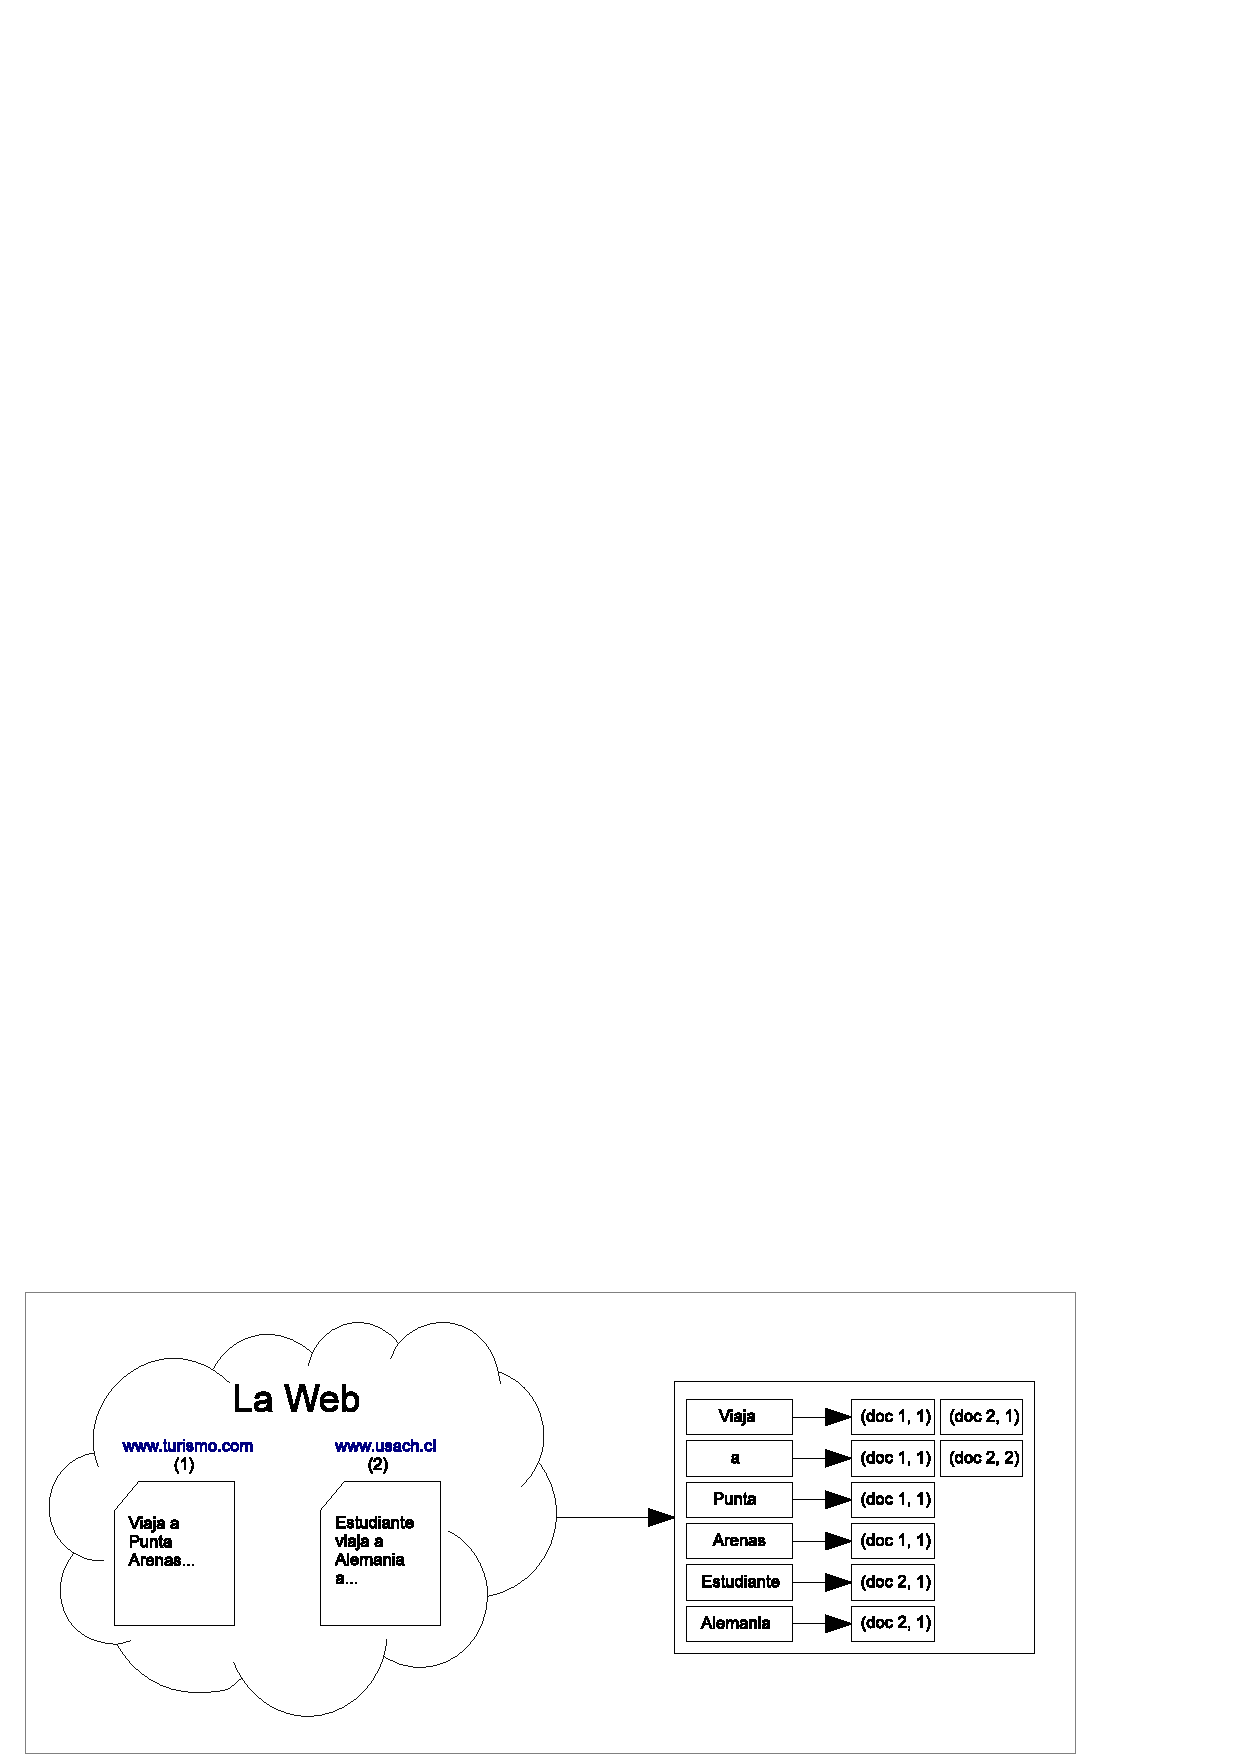
\includegraphics[scale=.75]{images/invertedindex.png}
\caption{\'Indice invertido}
\label{fig:invertedindex}
\end{figure}

El tamaño del índice invertido crece rápido y eventualmente la memoria RAM se agotará antes de procesar toda la colección de documentos. Cuando la memoria RAM se agota, se almacena en disco el índice parcial hasta aquel momento, se libera la memoria y se continúa con el proceso. Además, se debe hacer un \textit{merge} de los índices parciales uniéndo las listas invertidas de cada uno de los términos involucrados. Es por esto que se han desarrollado algunas técnicas de compresión con el objetivo de guardar de una manera más eficiente el índice invertido \citep{Arroyuelo:2013, Baeza-Yates:2011, Yan:2009}.

\section{Estrategias de evaluaci\'on de transacciones de lectura}
\label{marco:eeq}
Una de las tareas que un motor de búsqueda debe hacer para resolver una consulta es calcular el puntaje o \textit{score} para aquellos documentos relevantes en la consulta y así poder extraer los mejores $k$ documentos. Existen dos principales estrategias para recorrer las listas invertidas y calcular el puntaje de los documentos para una determinada consulta. Estas son (a) \textit{term-at-a-time} \citep{Buckley:1985, Turtle:1995} y (b) \textit{document-at-a-time} \citep{Broder:2003, Turtle:1995}.

\subsection{Term at a time}
Abreviada TAAT, este tipo de estrategia procesa los términos de las consultas una a una y acumula el puntaje parcial de los documentos. Las listas invertidas asociadas a un término son procesadas secuencialmente, esto significa que todos los documentos presentes en la lista invertida del término $t_{i}$ obtienen un puntaje parcial antes de comenzar el procesamiento del término $t_{i+1}$. La secuencialidad en este caso es con respecto a los términos contenidos en la transacción de lectura.

\subsection{Document at a time}
Abreviada DAAT, en este tipo de estrategias se evalúa la contribución de todos los términos de la \textit{query} con respecto a un documento antes de evaluar el siguiente documento. Las listas invertidas de cada término de la consulta son procesadas en paralelo, de modo que el puntaje del documento $d_{j}$ se calcula considerando todos los términos de la transacción de lectura al mismo tiempo. Una vez que se obtiene el puntaje del documento $d_{j}$ para la \textit{query} completa, se procede al procesamiento del documento $d_{j+1}$.

\subsection{Consideraciones}
Cuando se tiene un índice invertido pequeño, las estrategias TAAT rinden adecuadamente, sin embargo cuando los índices invertidos son de gran tamaño las estrategias DAAT poseen dos grandes ventajas: (a) Requieren menor cantidad de memoria para su ejecución, ya que el puntaje parcial por documento no necesita ser guardado y (b) Explotan el paralismo de entrada y salida (I/O) más eficientemente procesando las listas invertidas en diferentes discos simultáneamente. Además existen técnicas para optimizar el proceso de las estrategias recientemente descritas \citep{Turtle:1995}.



\section{Funciones de \textit{Ranking}}
\label{marco:ranking}
Los sistemas de recuperación de información como los motores de búsqueda deben ejecutar un proceso el cual asigna un puntaje a documentos con respecto a una determinada \textit{query}, este proceso se denomina \textit{ranking} \citep{Baeza-Yates:2011}. Como se puede ver en la Figura \ref{fig:ranking_process}, este proceso toma como entrada la representación de las \textit{queries} y documentos, y asigna un puntaje (\textit{score}) a un documento $d_{j}$ dada una \textit{query} $q_{i}$.

Un motor de búsqueda guarda billones de documentos que están formados por términos o palabras, estos términos no todos poseen la misma utilidad para describir el contenido del documento. Determinar la importancia de una palabra en un documento no es tarea sencilla, para ello se asocia un peso positivo $w_{i,j}$ a cada término $t_{i}$ del documento $d_{j}$. De esta forma, para un término $t_{i}$ que no aparezca en el documento $d_{j}$ se tendrá $w_{i,j} = 0$. La asignación de pesos a los términos permite generar un \textit{ranking} numérico para cada documento en la colección.


\begin{figure}[tp]
\centering
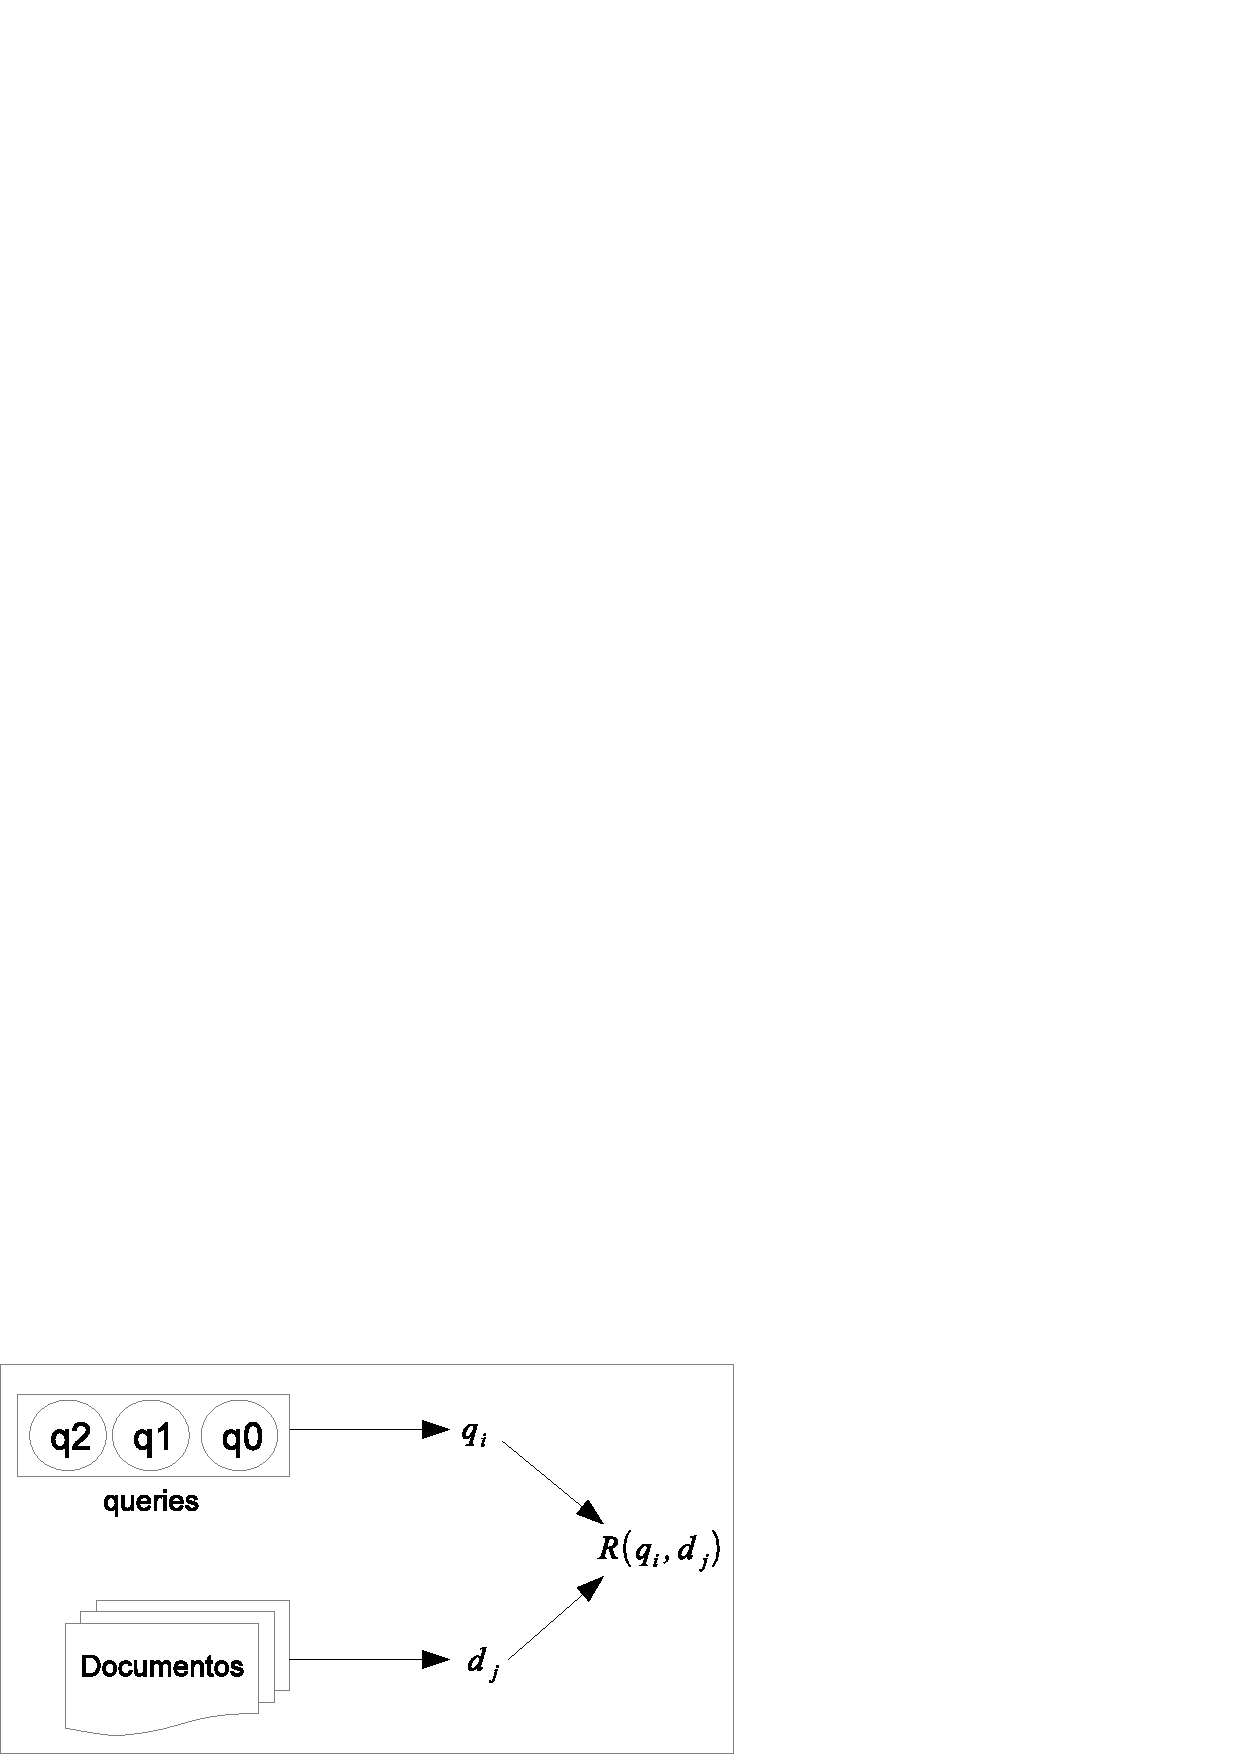
\includegraphics[scale=.75]{images/ranking_process.png}
\caption{Operaci\'on AND}
\label{fig:ranking_process}
\end{figure}


\subsection{TF-IDF}
\label{marco:tfidf}
El tf-idf (\textit{term frequency - inverse document frequency}) es un estadístico que tiene por objetivo reflejar cuán importante es una palabra para un documento en una colleción o corpus. Este estadístico se divide en dos partes, el primero corresponde a la frecuencia de la palabra o término en un documento (tf) y que en su versión más sencilla se utiliza la frecuencia bruta del término t en el documento d (f(t,d)). El segundo término corresponde a la frecuencia inversa de documento (idf) y se utiliza para observar si es que el término es común en el corpus. El idf obtiene calculando el logaritmo de la división entre el número total de documentos del corpus y el número de documentos que contienen el término.
De esta forma se tiene:

$$tf(t,d) = \dfrac{f(t,d) }{ max{f(w,d) : w \in d}}$$

$$idf(t,D) = log \frac{ |D| }{1 + |{d \in D : t \in d}|} $$

$$ tfidf(t,d,D) = tf(t,d) * idf(t,D) $$

Por lo que el estadístico \textit{TF-IDF} incrementa proporcionalmente al número de veces que la palabra aparece en el documento, sin embargo es compensado por la frecuencia de la palabra en la colección completa de documentos o corpus. Notar que la compensación ayuda a controlar el hecho de que algunas palabras son generalmente más comunes que otras.


\subsection{BM25}
\label{marco:bm25}
Es una función de \textit{ranking} de documentos basada en los términos que aparecen en la \textit{query} que llega al motor de búsqueda. \textit{BM25} pertenece a una amplia gama de funciones de puntuación y está basada en los modelos probabilísticos de recuperación de la información \citep{Baeza-Yates:2011}.

Dada una \textit{query} $Q$ que contiene los términos $q_{1},...,q_{n}$, el \textit{ranking BM25} del documento D se calcula como: 

$$ score(D,Q) =  \displaystyle\sum_{i=1}^n IDF(q_{i}) * \frac{f(q_{i},D)*(k+1)}{f(q_{i},D)+k * (1 - b + b * \frac{|D|}{prom(docs)})} $$

donde $f(q_{i}, D)$ es la frecuencia en que aparece el término $q_{i}$ en el documento D; $|D|$ es el número de palabras o términos en el documento D; $prom(docs)$ es la media de número de palabras de los documentos en el corpus; k y b son constantes que depende de las características del corpus en el que se está haciendo la búsqueda, por lo general se asignan los valores de $k = 2$ o $k = 1.2$ y $b = 0.75$; finalmente, $IDF(q_{i})$ es la frecuencia inversa de documento para el término $q_{i}$.


\section{Operaciones sobre listas invertidas}
\label{marco:osli}
Cuando una \textit{query} llega al motor de búsqueda, cada término tiene asociado una lista con todos los documentos en los cuales aparece. El sistema debe decidir qué documentos se analizarán para obtener la respuesa con el conjunto de los K mejores.
A continuación se presentan las diferentes formas de operar las listas invertidas de una \textit{query}.

\subsection{\textit{OR}}
\label{marco:or}
Este operador toma las listas invertidas de cada uno de los términos de la \textit{query} y ejecuta la disyunción entre ellas. El resultado de este operador es una lista invertida con todos los documentos que contengan al menos un término de la \textit{query}. Finalmente, esta lista invertida se ocupará para obtener los mejores K documentos. Un simple ejemplo se muestra en la FIGURA \ref{fig:ORoperation}.

\begin{figure}[tp]
\centering
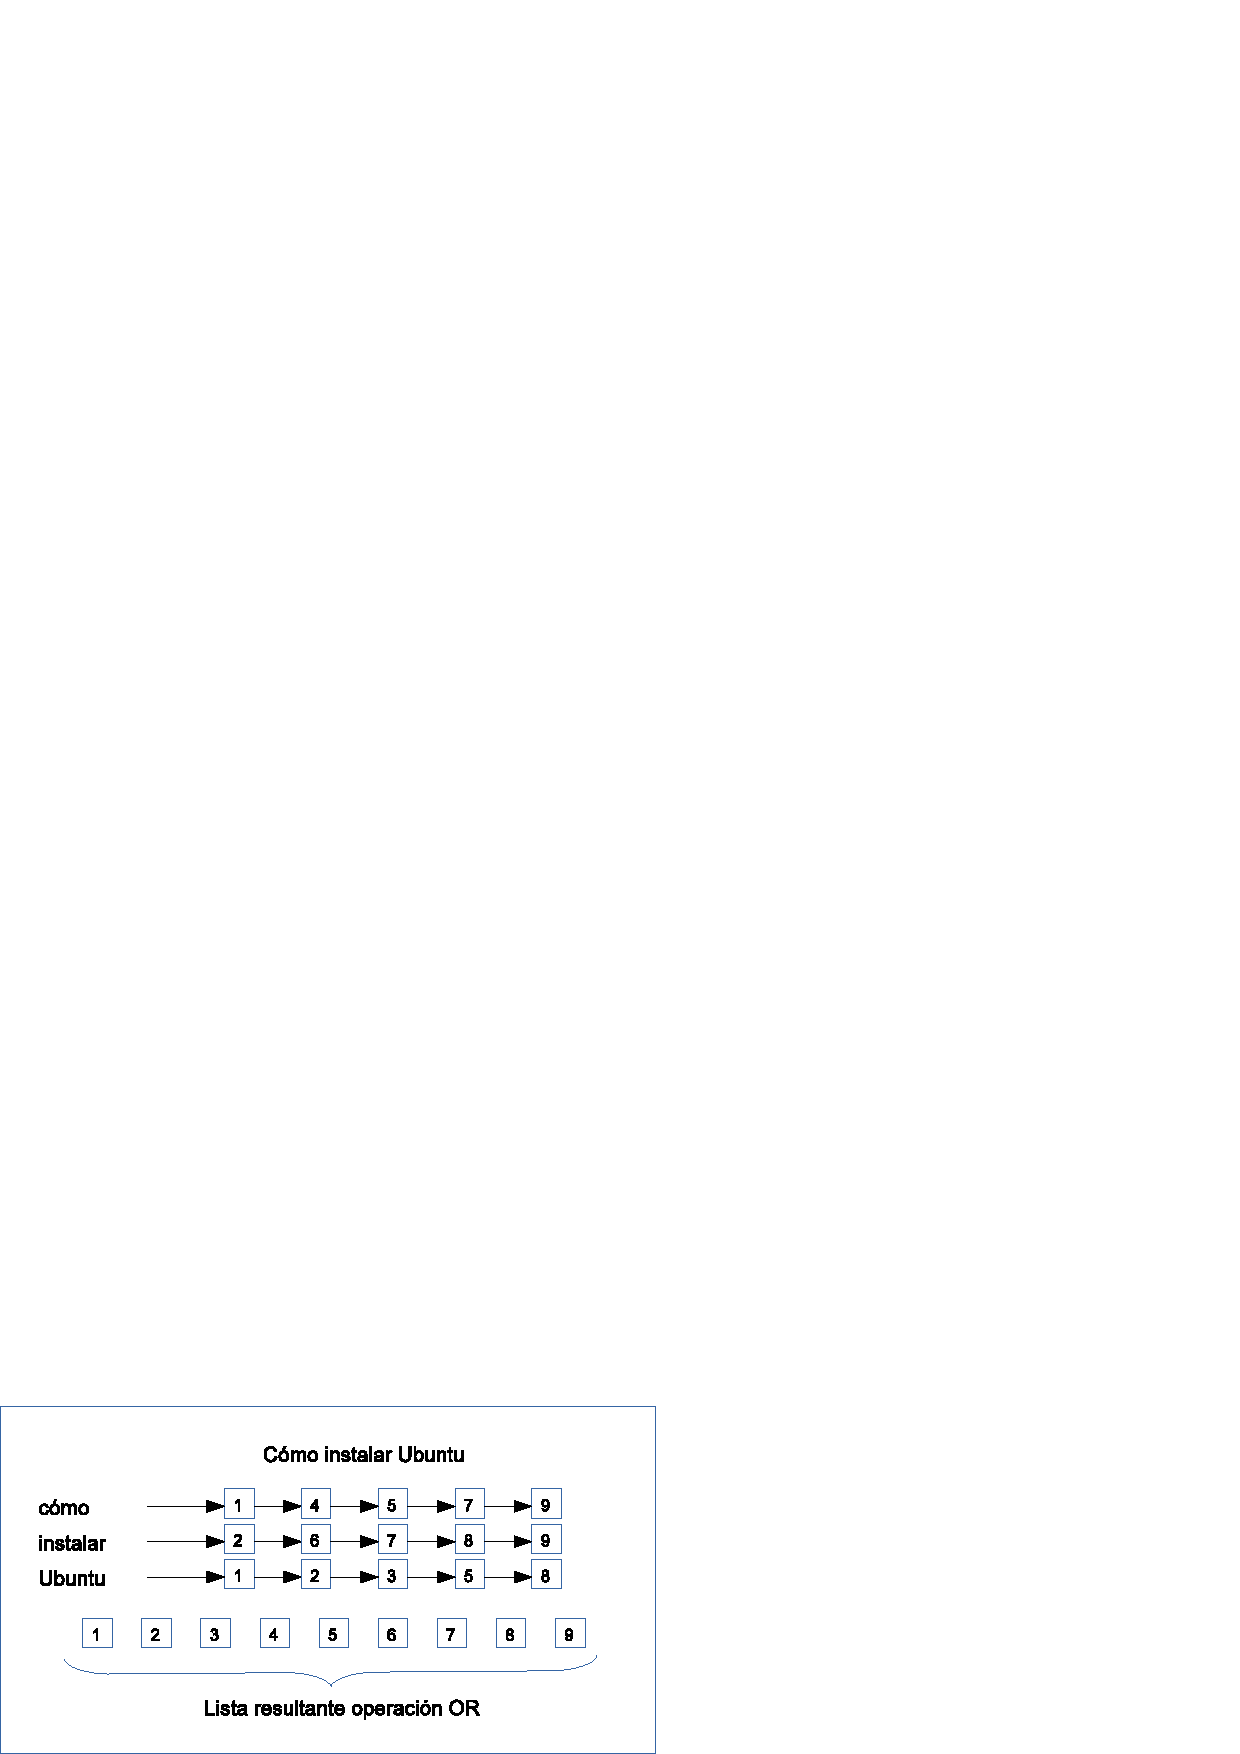
\includegraphics[scale=.75]{images/ORoperation.png}
\caption{Operaci\'on OR}
\label{fig:ORoperation}
\end{figure}

\subsection{AND}
\label{marco:and}
Este operador ejecuta la conjunción entre las listas invertidas de los términos de una \textit{query}. Se obtiene una lista invertida con los documentos que contengan todos los términos de la \textit{query}. Se debe notar que aquí se obtiene una lista resultante de menor tamaño que la obtenida en el operador OR (Ver FIGURA \ref{fig:ANDoperation}).

\begin{figure}[tp]
\centering
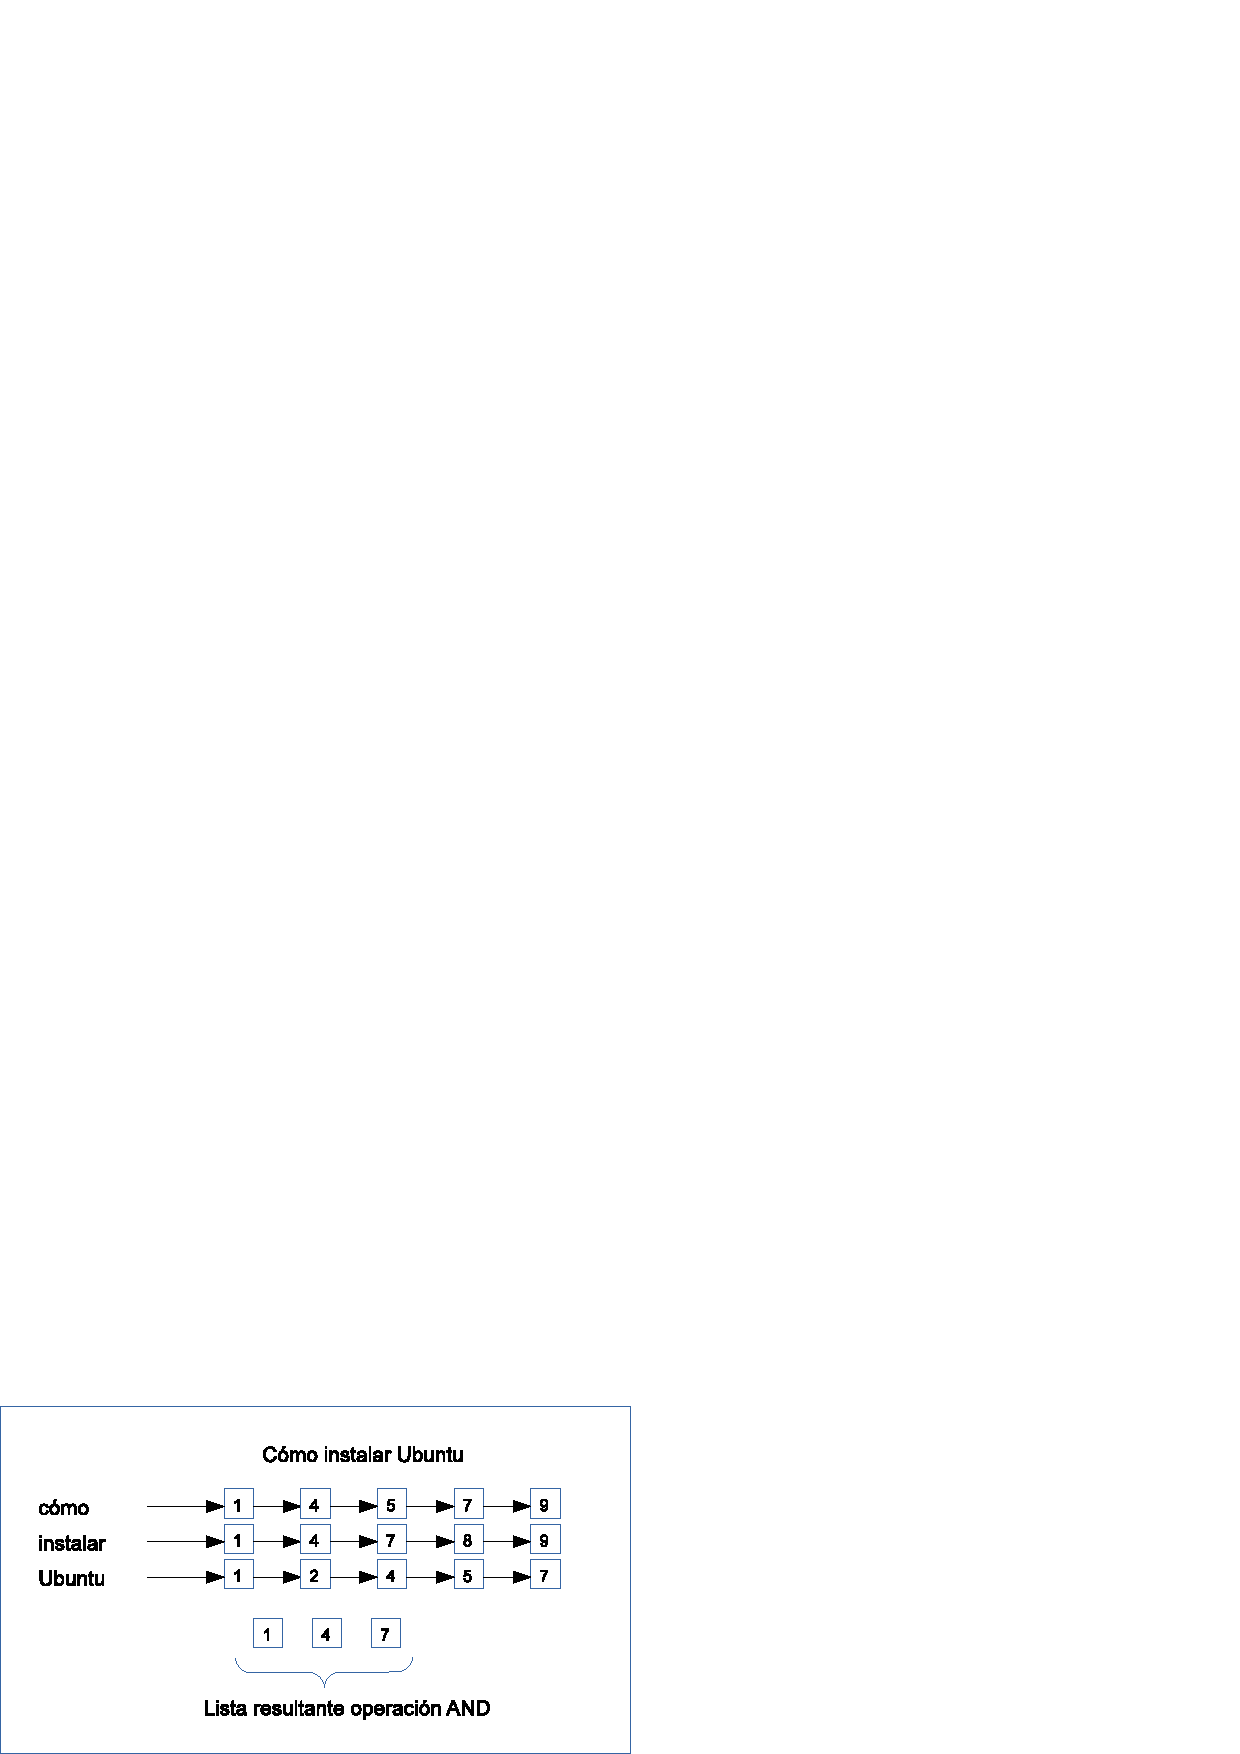
\includegraphics[scale=.75]{images/ANDoperation.png}
\caption{Operaci\'on AND}
\label{fig:ANDoperation}
\end{figure}


\subsection{WAND}
\label{marco:wand}
Algoritmo de evaluación de transacciones de lectura para obtener eficientemente el conjunto de K documentos que mejor satisfacen una \textit{query} dada. \textit{WAND} \citep{Broder:2003} es un proceso menos estricto que el método \textit{AND} y está basado en dos niveles. Dentro del proceso de evaluación de una transacción de lectura, uno de los procesos más costoso en términos de tiempo es el de \textit{scoring}, que consiste en entregarle a cada uno de los documentos analizados un puntaje que representa la relevancia del documento para una \textit{query} dada, esto se denomina evaluación completa o cálculo del puntaje exacto del documento. El objetivo de WAND es minimizar la cantidad de evaluaciones completas de los documentos ejecutando un proceso de dos niveles. En el primer nivel se intenta omitir rápidamente grandes porciones de las listas invertida, lo que se traduce en ignorar el cálculo del puntaje exacto de grandes cantidades de documentos, esto porque en motores de búsqueda a gran escala, este un proceso que requiere de mucho tiempo para llevarse a cabo y depende de factores como la cantidad de ocurrencia del término dentro del documento, el tamaño del documento, entre otros.  

Para llevar a cabo el algoritmo WAND y así reducir el número de documentos completamente evaluados durante el proceso de \textit{ranking} de documentos, se necesita calcular los valores estáticos de límite superior (\textit{upper-bounds}), en donde para cada uno de los términos del índice invertido, se toma la lista invertida correspondiente y se extrae el puntaje máximo de contribución de algún documento con respecto al término. El cálculo de los \textit{upper bounds} se lleva a cabo cuando se construye el índice invertido y en donde a cada término del índice se asocia el puntaje máximo que existe en la lista invertida. 

WAND usa un índice invertido ordenado por los identificadores de documentos. En el primer nivel se itera sobre los documentos del índice invertido de cada término y se identifica los potenciales candidatos usando una evaluación aproximada. En el segundo nivel, aquellos documentos candidatos son completamente evaluados y su puntaje exacto es calculado. De esta forma se obtiene el conjunto final de documentos. Se utiliza un heap como estructura de datos para almacenar el conjunto de los mejores K documentos, en donde el elemento superior corresponde al documento con menor puntaje y es el que se utilizará como umbral (\textit{threshold}) para decidir si los siguientes documentos deben ser completamente evaluados o no. 

En la Figura \ref{fig:proceso_wand} se puede ver un ejemplo sencillo de cómo el algoritmo Wand trabaja en la resolución de una transacción de lectura de tres términos: 'casa', 'perro' y 'gato'. Como la \textit{query} está compuesta por tres términos, existen tres punteros que recorren cada una de las listas invertidas (notar que cada puntero recorre una lista invertida diferente). Lo primero que se hace es ordenar las listas invertidas de acuerdo a los identificadores de documentos que se están apuntando, razón por la cual en la Figura \ref{fig:proceso_wand} la lista invertida de 'casa' (puntero referenciando al documento con identificador 125), aparece primero que la lista invertida de 'perro' (puntero haciendo referencia al documento con identificador 503). Luego se suma los \textit{uppers bounds} de los términos en orden hasta que se obtiene un valor mayor o igual al \textit{threshold}. De esta manera el término 'perro' es escogido como término pivote ($2.0 + 4.4 >= 5.7$) y el actual documento al cual se está apuntando es escogido como documento pivote (documento con identificador 503). Si las dos primeras listas invertidas no contienen el documento 503 entonces se procede a seleccionar el siguiente pivote, en otro caso se calcula el puntaje completo del documento. Finalmente, si el puntaje es mayor o igual al threshold, se actualiza el heap eliminando el elemento superior y se añade el nuevo documento. 
Este algoritmo es repetido hasta que no hayan más documentos a procesar o hasta que no exista un documento que supere el actual threshold. De esta manera se evita procesar las listas completas \citep{Blanco:2010}.

\begin{figure}[H]
\centering
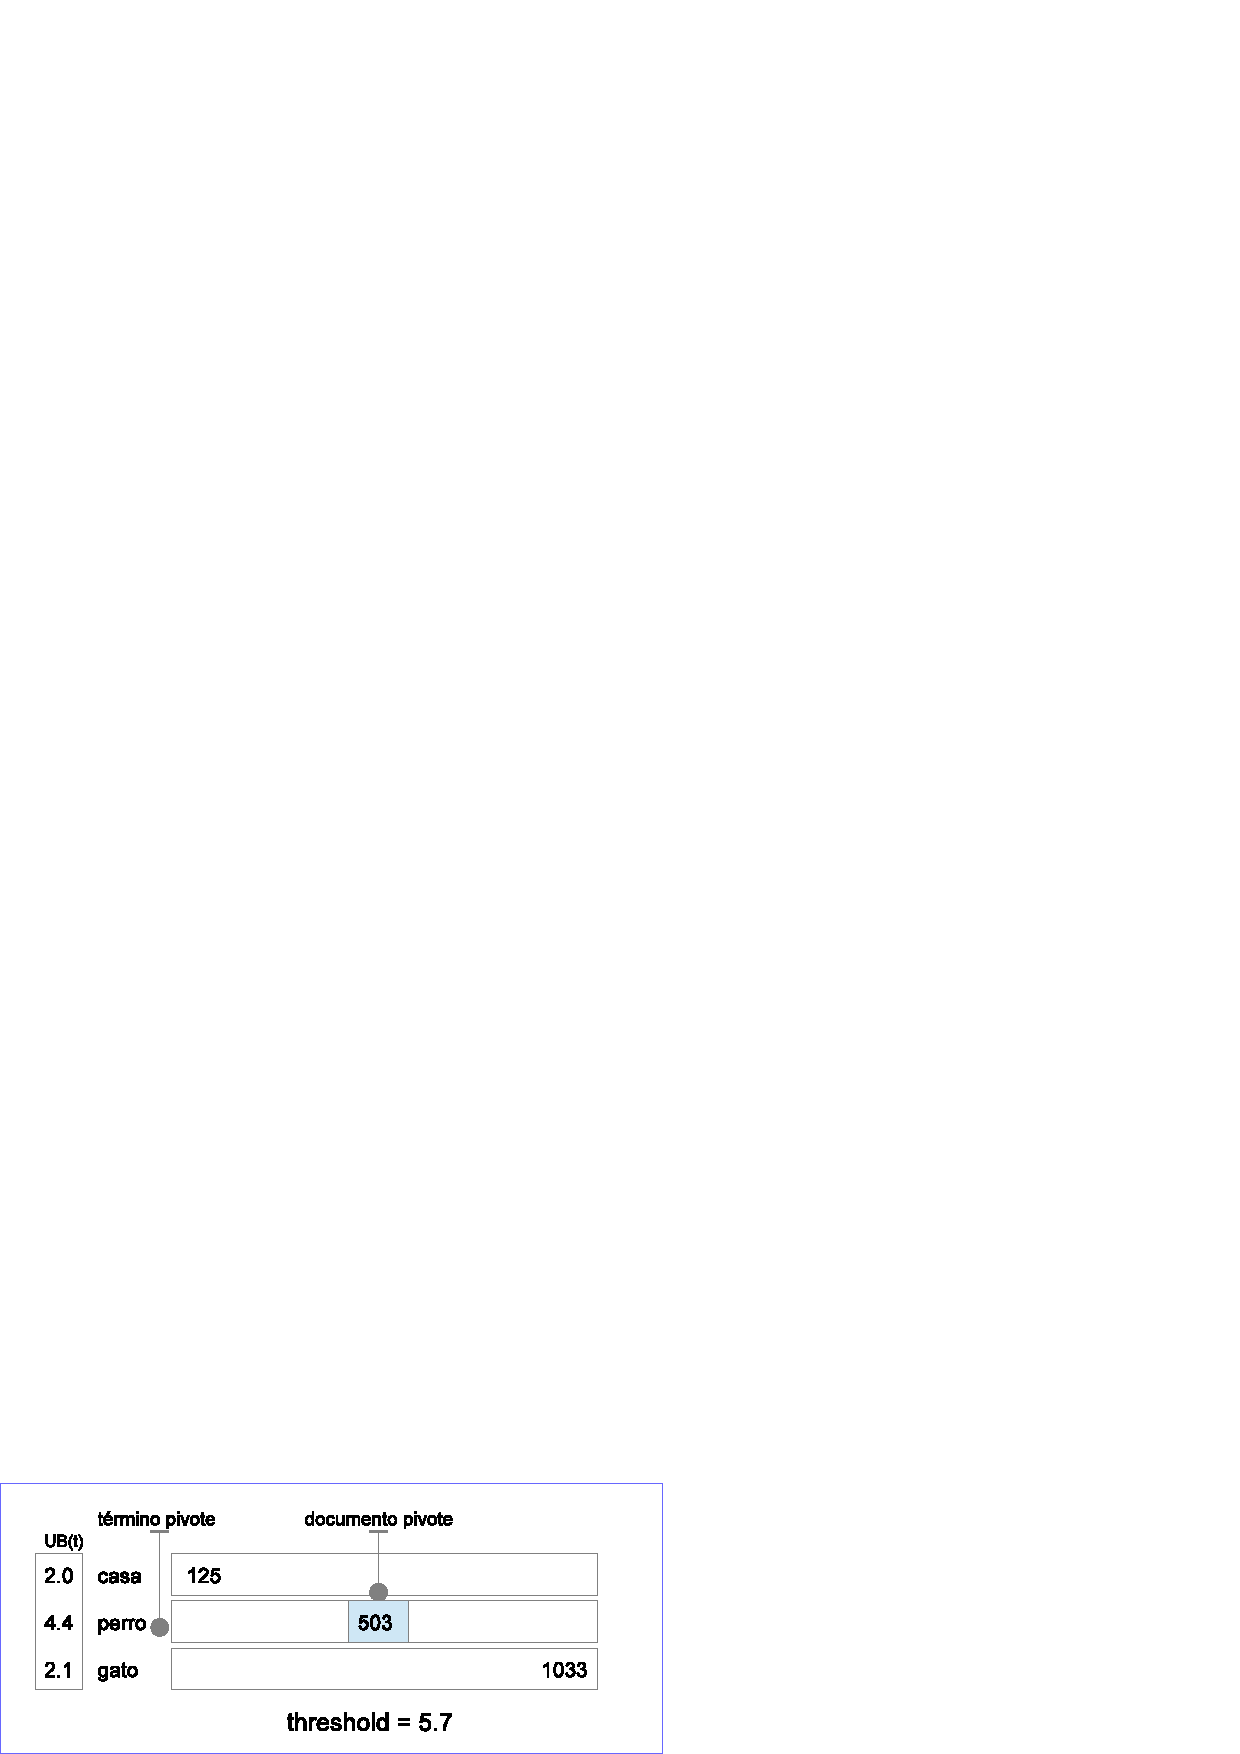
\includegraphics[scale=.75]{images/proceso_wand.png}
\caption{Ejemplo de ejecución de algoritmo  \textit{Wand}}
\label{fig:proceso_wand}
\end{figure}


\section{Scheduling en motores de búsqueda}
\label{marco:scheduling}
Los sistemas de recuperación de la información como los motores de búsqueda, no solo se preocupan de la calidad de los resultados de las búsquedas (efectividad), sino que también de la velocidad con la que los resultados son obtenidos (eficiencia). Existen varias estrategias para mejorar la velocidad en la obtención de los resultados, una de ellas muy utilizada es el \textit{caching}. Consiste en guardar en memoria de acceso rápido (memoria caché) datos temporales, que luego pueden ser sobrescrito. Una opción es hacer \textit{caching} de los resultados de las búsquedas, de esta forma cuando una \textit{query} es encontrada en caché el motor de búsqueda puede generar la respuesta rápidamente, reduciendo los tiempos de calculos considerablemente. Otra opción es, guardar en caché la intersección de las listas invertidas de pares comunes de términos que llegan al motor de búsqueda. Por ejemplo, si llega al sistema una consulta con los términos ('casa', 'árbol', 'perro'), se puede guardar en caché la intersección de las listas de 'casa' y 'árbol', para luego reutilizar esta información en otras \textit{queries} que lleguen en el futuro. Para ver más técnicas de \textit{caching} y ver el detalle de las técnicas mencionadas, ver \citep{Buttcher:2010}.

Otra estrategia para acelerar el proceso de resolución de \textit{queries} que llegan al sistema es el uso de algoritmos de planificación (scheduling). Un algoritmo de \textit{scheduling} es el proceso en el cual se cambia el orden en que llegan las \textit{queries} al motor de búsqueda con el objetivo de mejorar la eficiencia. 

Existen dos clases de algoritmos de \textit{scheduling}, estáticos y dinámicos. Los estáticos son aquellos en que se conoce el conjunto completo de tareas y las características de cada una de ellas, como por ejemplo, el tiempo de procesamiento. Los algoritmos de \textit{scheduling} dinámicos son aquellos en que no se conoce las tareas que llegarán en el futuro, también se desconoce el momento en que éstas llegarán. La filosofía de los algoritmos de \textit{scheduling} dinámicos es ajustarse a los cambios que pueden haber en el sistema.

En el contexto del presente trabajo de tesis, el objetivo de hacer \textit{scheduling} es minimizar el tiempo en que las \textit{queries} son procesadas por un motor de búsqueda. Los motores de búsqueda como \textit{Google}\footnote{http://www.google.com} o \textit{Yahoo!}\footnote{http://www.yahoo.com} trabajan en un contexto \textit{online}. Esto significa que cuando las \textit{queries} llegan al sistema (una a una), éste está obligado a tomar una decisión para planificarla sin saber cuáles \textit{queries} llegarán en un momento posterior. A esto se le conoce como algoritmo de \textit{scheduling online} \citep{Albers:2003, Borodin:1998}.

Los sistemas IR a gran escala despliegan una arquitectura distribuída \citep{Dean:2009}, en donde el índice invertido está particionado \citep{Barroso:2003} a lo largo de servidores (\textit{shard servers}), los cuales están encargados de procesar las \textit{queries} que llegan al sistema. Es fácil notar que resolver una \textit{query} con varios \textit{shard servers} mejoraría la eficiencia. Ahora bien, para asegurar un alto rendimiento (\textit{throughput}) del sistema, cada uno de los \textit{shard servers} posee réplicas, de esta forma, más \textit{queries} pueden ser procesadas en paralelo en copias idénticas del mismo \textit{shard server}. Esto implica que el tiempo de espera de las \textit{queries} que vienen llegando al sistema se reduce. 

Como en un sistema con arquitectura como el de la Figura \ref{fig:sistemaIR}, una \textit{query} puede ser procesada por varios \textit{shard servers}, el \textit{broker} debe escoger la réplica más apropiada para procesar la parte de la \textit{query} asignada al \textit{shard server}, con el objetivo de reducir el tiempo de espera de ésta. El \textit{broker} podría seleccionar el \textit{shard server} con el menor número de \textit{queries} en la cola, sin embargo, este no es un parámetro adecuado, ya que el tiempo de respuesta de las \textit{queries} puede variar considerablemente, especialmente si se usa poda dinámica \citep{Broder:2003, Moffat:1996}. 


\begin{figure}[tp]
\centering
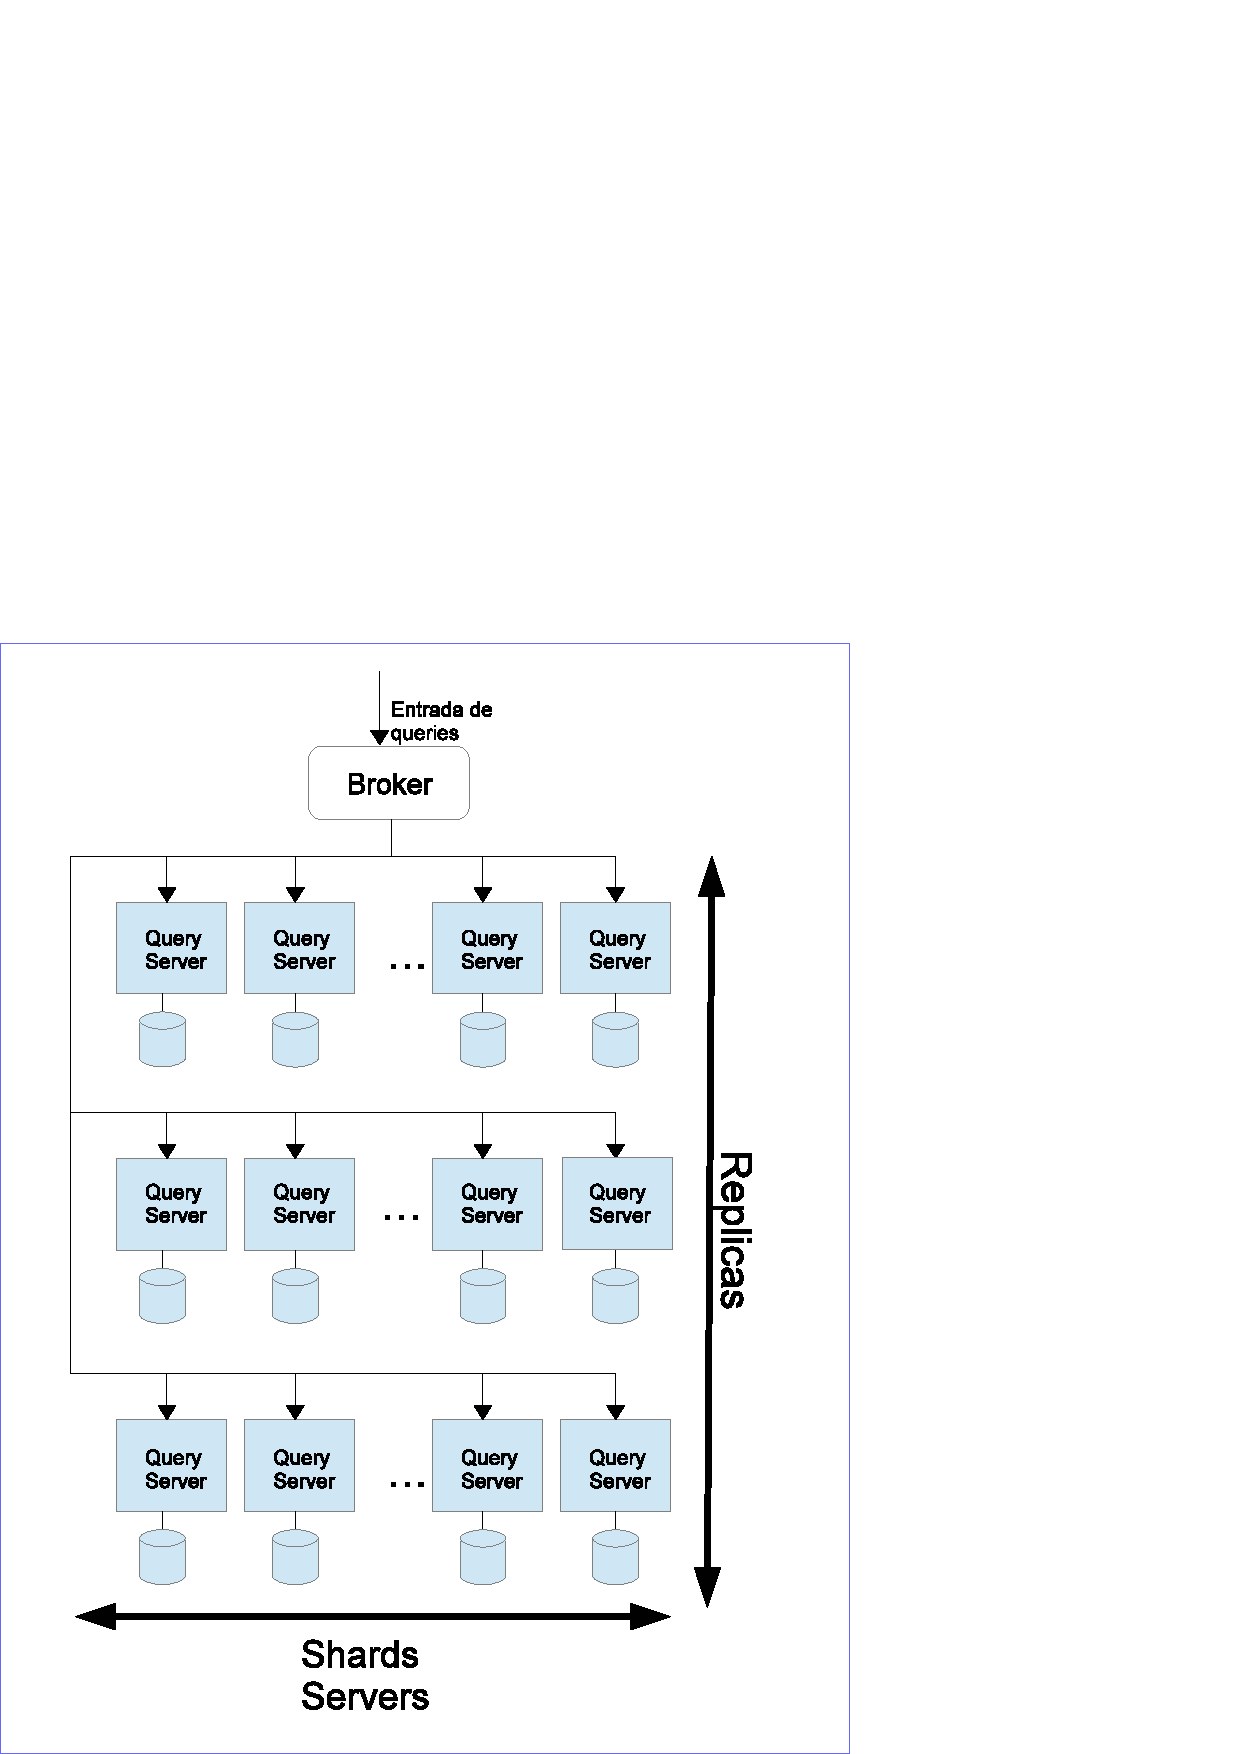
\includegraphics[scale=.75]{images/sistemaIR.png}
\caption{Arquitectura de un sistema de recuperación de la información con réplicas}
\label{fig:sistemaIR}
\end{figure}

\subsection{Trabajo relacionado}
\label{marco:tr}
El estudio \citep{Broccolo:2013} analiza métodos de \textit{dropping} y \textit{stopping} para el procesamiento de \textit{queries} bajo altas carga de trabajo en un sistema distribuído donde existen múltiples servidores en el que cada uno resuelve una parte de la \textit{query} para luego enviar las consultas al \textit{broker} y éste hace el \textit{merge} de los resultados de acuerdo al \textit{score} de los documentos. Se define un tiempo \textit{T}, en el que la suma de el tiempo de espera de la \textit{query} para ser procesada ($t_{w}$) y el tiempo de procesamiento de la misma ($t_{p}$) deben ser menor a \textit{T}. Si es que se sobrepasa este tiempo, se tienen dos opciones (1) la \textit{query} es desechada y se envía al \textit{broker} una lista vacía, (2) se detiene el procesamiento de la \textit{query} y se envía los resultados parciales hasta el momento. Finalmente se propone un método basado en la predicción de tiempo de respuesta ($\hat{pt}(q)$) de una \textit{query} \citep{Macdonald:2012} de modo que si se cumple $ \hat{pt}(q) \leq T - wt(q) $, entonces la \textit{query} es desechada antes de comenzar a procesarse y se toma la siguiente desde la cola de espera. Notar que en estos métodos existe una pérdida de efectividad, puesto que eventualmente los servidores muchas veces no enviarán sus mejores documentos al \textit{broker}, esto implica que el \textit{broker} responderá al usuario un conjunto de K documento que no necesariamente son los mejores dentro del corpus completo.

En \citep{Freire:2012} se estudia el impacto que tiene la técnica de predicción de tiempos de respuestas para \textit{queries}, \citep{Tonellotto:2011} en sistemas de recuperación de la información con réplicas. En este estudio, se llega a la conclusión que usando una buena predicción, se puede reducir el tiempo que la \textit{query} tiene que esperar para ser procesada ($t_{w}$), y también se puede reducir el tiempo total requerido para procesar el conjunto (\textit{log}) completo de \textit{queries} (\textit{completion time}). En \citep{Freire:2013}, se propone un modelo híbrido de \textit{scheduling} de \textit{queries} a través de réplicas, en el que cuando el sistema se encuentre bajo altas cargas de trabajo, se utilice política de \textit{scheduling} basada en la predicción de tiempo de respuesta de las \textit{queries} \citep{Macdonald:2012} y cuando el sistema se encuentre con una baja carga de trabajo, se utilice una politica de \textit{scheduling} sencilla y de menor costo como \textit{Round Robin}.
\chapter{Wand \textit{multi-threaded}}
\label{cap:wand}

Dado que el método WAND \citep{Broder:2003} consiste es el método del estado del arte ocupado hoy en día por los motores de búsqueda, en esta investigación se asume un sistema que usa este método para obtener eficientemente los mejores K documentos a una transacción de lectura. Este algoritmo usa un \textit{ranking} basado en una evaluación de dos niveles. En el primer nivel, este usa una cota superior (\textit{upper bound}) al puntaje de cada documento para intentar descartarlos eficientemente. En el segundo nivel se computa el puntaje real de los documentos que pasa el primer nivel. Se utiliza una estructura de datos llamada \textit{heap} que va guardando el conjunto de los mejores K documentos hasta un determinado instante. El menor puntaje de este conjunto es usado como umbral (\textit{threshold}) para las evaluaciones del primer nivel, de esta forma se descarta rápidamente documentos que no pueden ser parte del conjunto final de los \textit{top-K} documentos. Esto permite un eficiente y a la vez seguro proceso de descarte que asegura que en el resultado final se encontrará el conjunto correcto y no se perderán documentos relevantes.

Existen dos formas de implementar Wand \textit{multithreaded}. Una de ellas es usando \textit{heaps} locales (LH), es decir, un \textit{heap} por hilo de ejecución (\textit{thread}) y el otro es usando \textit{heaps} compartidos (SH). El estudio en \citep{Rojas:2013} se muestra indicios que el esquema SH es generalmente más eficiente. Logrando rápidamente un óptimo valor para el threshold, el esquema SH posee las siguientes ventajas: (1) Se puede reducir el número de calculo de puntajes completos y (2) se ejecutan pocas operaciones de actualización del heap (reduciendo el número de \textit{locks} que se hace a la estructura de dato). A continuación se presenta el diseño llevado a cabo para ambos esquemas.

\section{Block max wand}
Recordar que en el método de Wand para descartar documentos y encontrar un documento que potencialmente podría estar en el conjunto \textit{top-K}, lo que se hace es usar los \textit{upper bounds} globales de cada lista, es decir, la máxima contribución (puntaje o \textit{score}) de algún documento de la lista invertida. Además, Wand tradicional es una estrategia DAAT, por lo que por cada lista invertida ocupa un puntero al documento actual que se desea evaluar. Además, usa un método que recibe como entrada un identificador del documento $docID$ y una lista invertida $L$, y retorna el primer $docID'$ que sea mayor o igual al documento $docID$. A esto se le conoce como movimiento de puntero profundo (\textit{deep pointer movement}) debido a la razón que generalmente implica una descompresión del boque en el que se encuentra el documento.

Sin embargo, como se dijo anteriormente en \ref{marco:bmw}, usando solo las máximas contribuciones por cada bloque no hará que el método funcione correctamente, puesto que hará que eventualmente se pierdan documentos que podrían estar en el conjunto final de los mejores $K$ documentos. Como ahora se tiene las máximas contribuciones por cada bloque, BMW utiliza otra función la cual recibe como parámetro un identificador de documento $docID$ y una lista invertida. Lo que se hace es mover el puntero actual al correspondiente bloque donde eventualmente se debería encontrar el documento $docID$. A esta función se le conoce como movimiento de puntero superficial (\textit{shallow pointer movement}), por la razón que no involucra una descompresión de bloque. Se debe notar que para que esta función trabaje correctamente se requiere tener almacenada las fronteras de cada uno de los bloques de las listas invertidas.

BMW utiliza dos principales ideas en su diseño: (1) Se usa los \textit{upper bounds} globales para determinar un pivote candidato (como en Wand tradicional), para luego usar los \textit{upper bounds} locales para determinar si es que el pivote candidato es un pivote real o no, y (2) Se intenta siempre utilizar \textit{shallow pointer movement} por sobre \textit{deep pointer movement}.

En el Algoritmo \ref{alg:bmw} se puede apreciar cómo el método \textit{Block-Max-Wand} trabaja. Recordar que todas las listas invertidas poseen un puntero al documento actual que se desea evaluar (\textit{currentDoc}). Lo primero que se hace es ordenar en orden creciente las listas invertidas de acuerdo a su correspondiente \textit{currentDoc}. La función \textit{findPivot()} es la misma que se utiliza en el método Wand tradicional (\ref{marco:wand}), se itera sobre las listas invertidas y se retorna la posición de la lista en donde se cumple que la suma de los \textit{upper bounds} globales es mayor al \textit{threshold} ($\theta$). Luego la función \textit{NextShallow()} se encarga de avanzar los punteros de las listas invertidas al inicio del bloque que debería contener el documento $d$. Posteriormente la función \textit{isRealPivot()} verifica si es que el pivote $p$ encontrado es un pivote real o no, para cada una de las listas desde la posición $0$ hasta la posición $p$, se suma los \textit{upper bounds} de los bloques en donde se encuentran los punteros (recordar que con \textit{NextShallow()} los punteros de las listas quedaron apuntando a los bloques en donde se debería encontrar el documento $d$), si la suma es mayor al threshold entonces retorna verdadero, de lo contrario retorna falso. El método \textit{scoreDoc()} calcula el puntaje del documento que se le pasa por parámetro. 

Cuando el método se da cuenta que $p$ no es un pivote real, lo que se hace es buscar un nuevo candidato a través de la función \textit{getNewCandidate()}, la cual hace avanzar los punteros de las listas invertidas hasta el bloque siguiente que contenga el mínimo $docID$. Para ver explicar de mejor manera esta idea se presenta la Figura \ref{fig:getNewCandidate}, aquí se puede ver que el documento $4868$ es el pivote, cuando este documento no es un pivote real (la función \textit{isRealPivote} retorna falso), lo que se hará es escoger un documento $d'$ tal que $d = min(d1,d2,d3,d4)$ en donde $d1,d2,d3$ son la frontera del bloque actual más uno (inicio del bloque siguiente) y $d4$ es el \textit{currentDoc} de la cuarta lista. Notar que para hacer un descarte seguro de documentos, siempre se debe incluir a la elección del nuevo candidato el \textit{currentDoc} de la lista inmediatamente siguiente a la lista pivote (en este caso 9009).  

\begin{figure}[!th]
\centering
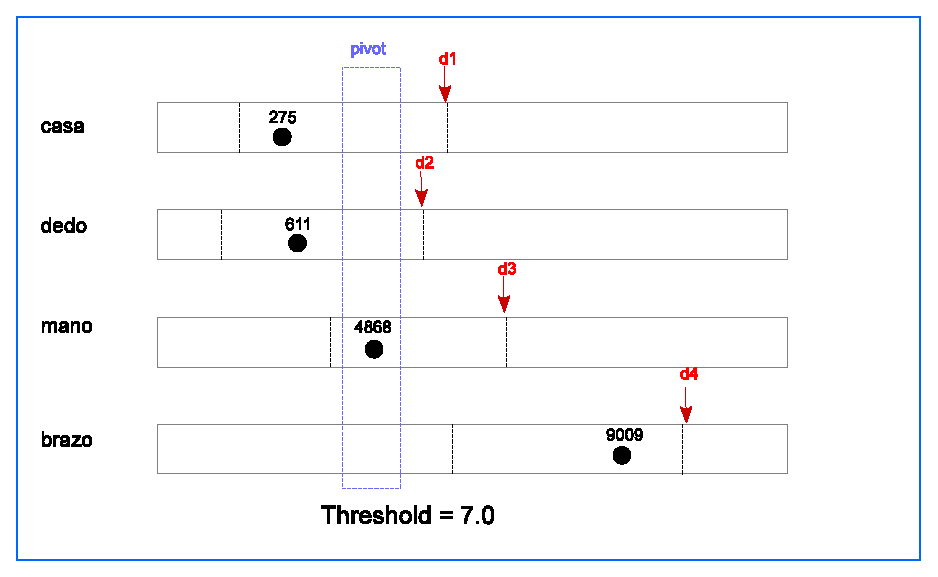
\includegraphics[scale=.75]{images/get_new_candidate.eps}
\caption{Ejemplo de cómo opera la functión getNewCandidate()}
\label{fig:getNewCandidate}
\end{figure}%y


\begin{algorithm}[!th]
\caption{\em $BMW(\theta, L, docID)$: Block Max Wand}
\label{alg:bmw}
\begin{algorithmic}[1]
\REQUIRE Un \textit{threshold} $\theta$, listas invertidas $L$ de los términos en la consulta
\ENSURE $docID$, si existe un documento $docID$ tal que $score(docID)$ $\geq$ $\theta$. de lo contrario END-OF-FILE
\WHILE {true}
	\STATE $Sort(L);$
	\STATE $p = findPivot(L,\theta);$
	\STATE $d = L[p] \rightarrow currentDoc;$
	\IF {$d == $ END-OF-FILE}
  		\STATE $break;$
	\ENDIF
		
	\FOR {$ i = 0...p $}
		\STATE $NextShallow(d, L[i]);$
	\ENDFOR
	
	\IF {$isRealPivot(\theta, p);$}
		\IF {$L[0] \rightarrow currentDoc == d$}
			\STATE $scoreDoc(d, p);$
			\FOR {$ i = 0...p $}
				\STATE $Next(d + 1, L[i]);$
			\ENDFOR
		\ELSE
			\WHILE {$List[p - 1] \rightarrow currentDoc == p $}
				\STATE $p = p - 1;$			
			\ENDWHILE
			
			\FOR {$ i = 0...p $}
				\STATE $Next(d, L[i]);$
			\ENDFOR
			
		\ENDIF		
	\ELSE	
		\STATE $d' = getNewCandidate();$
		\FOR {$ i = 0...p $}
			\STATE $Next(d', L[i]);$
		\ENDFOR
	\ENDIF
	
\ENDWHILE

\end{algorithmic}
\end{algorithm}

\section{Wand con heaps locales}
En el esquema LH, cada \textit{thread} procesa una porción del índice invertido mientras mantiene un \textit{heap} local con los mejores $K$ documentos que el específico hilo de ejecución ha encontrado hasta ahora. Al final del proceso, los resultados deben ser reunido en un solo conjunto final global. Los resultados en \citep{Rojas:2013} muestran que el esquema LH es más eficientes para aquellas transacciones que toman poco tiempo en ser resueltas. En la Figura \ref{fig:wand-heap-local} se muestra el esquema de ejecución para \textit{heaps} locales explicado anteriormente. 

\begin{figure}[!ht]
\centering
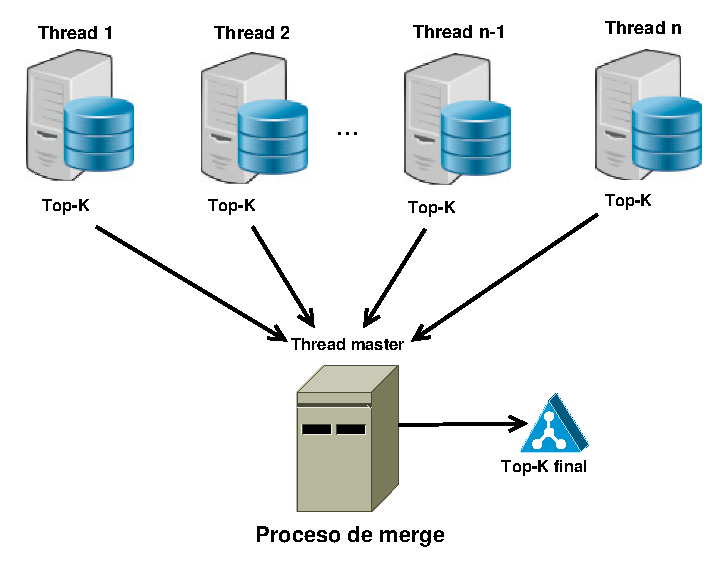
\includegraphics[scale=.75]{images/wand_heaps_locales.eps}
\caption{Esquema de ejecución de algoritmo WAND con heaps locales}
\label{fig:wand-heap-local}
\end{figure}

El diseño aplicado para implementar el esquema LH se puede ver en la Figura \ref{fig:TopKMultiThreadWandOperatorLocal}. La clase principal es la TopKMultiThreadWandOperatorLocal, que es la encargada de controlar el paralelismo en la resolución de las transacciones. Para explicar de mejor manera cada una de las clases involucradas en la implementación, se presenta el siguiente diccionario de datos.

\begin{figure}[!ht]
\centering
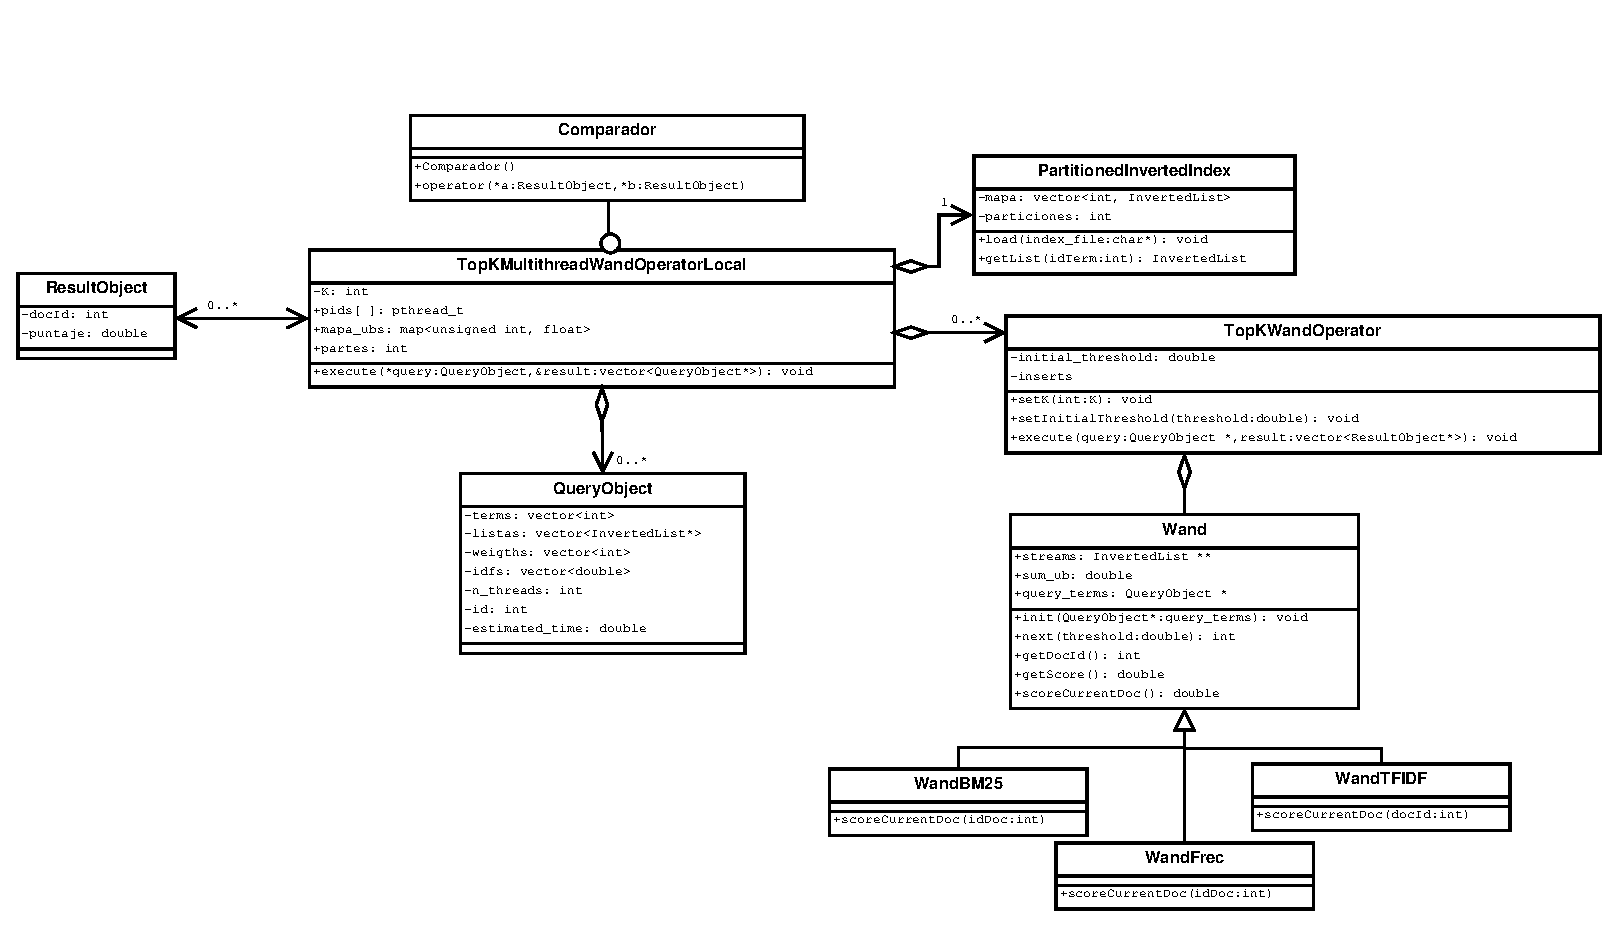
\includegraphics[scale=.75]{images/TopKMultiThreadWandOperatorLocal.eps}
\caption{Diagrama de clases para el esquema LH}
\label{fig:TopKMultiThreadWandOperatorLocal}
\end{figure}

\begin{list}{}{}
	\item \textbf{TopKMultiThreadWandOperatorLocal}. Clase encargada de devolver los mejores K documentos para una query dada. Si es que la query debe ser resuelta en forma paralela, esta clase además debe controlar el paralelismo que se produce en la resolución de ésta, inicializando las variables correspondientes para lanzar los hilos de ejecución y luego escogiendo los mejores documentos desde todos los heaps creados por los diferentes threads (proceso de merge). En esta clase se define un mapa que asocia cada término del índice invertido con el puntaje del mejor documento en esa lista invertida (upper bound de la lista invertida) y además se define cuántos documentos se van a retornar al final del proceso (atributo K). El método execute inicializa las variables locales para los diferentes threads, posteriormente hace el llamado al método \emph{thread-execute} (en el cual se llevará a cabo la resolución de la transacción de lectura en forma paralela), finalmente se toman los resultados parciales de cada uno de los hilos de ejecución y se ejecuta el proceso que mezcla los resultados, retornando solo los mejores K documentos. 
	
	\item \textbf{PartitionedInvertedIndex}. Clase que tiene la tarea de almacenar el índice invertido y extraer desde aquí las listas invertidas de documentos para cada uno de los términos de las transacciones de lectura. El almacenamiento el índice se lleva a cabo mediante un mapa cada término su lista invertida correspondiente y para la extracción de estas listas se usa el método getList.
	
	\item \textbf{TopKWandOperator}.  Cada thread tendrá su propio objeto TopKWandOperator encargado de obtener los mejores K documentos. El cálculo de este conjunto se realiza en el método execute con la ayuda de un objeto de tipo Wand asociado.
	
	\item \textbf{Wand}. Clase que controla la lógica del algoritmo wand. Lleva a cabo el proceso de inserción de documentos en el heap y todo lo que esto conlleva. Existen diferentes tipos de objetos Wand que se pueden utilizar, entre ellos están WandBM25, WandFrec y WandTFIDF, donde la única diferencia entre ellos es el método de que calcula el puntaje de cada documento. Por ejemplo, WandBM25 utiliza BM25 (citar) y WandTFIDF utiliza tf-idf (citar también). 
	
	\item \textbf{ResultObject}. Clase que se utiliza para guardar los mejores K documentos.
	
	\item \textbf{QueryObject}. Clase que representa una transacción de lectura. Está constutuída sus términos,  las respectivas listas invertidas y pesos de cada uno de ellos, la cantidad de threads con los cuales se resolverá dicha transacción y el tiempo estimado de procesamiento (este tiempo se predice al momento de resolver la query).

\end{list}




\section{Wand con heap compartido}
\label{scheduling:whc}
En el esquema SH cada thread procesa una porción del índice. Sin embargo, ahora un solo heap es creado y accedido por todos los threads. En este caso no se requiere de mezclar los resultados y el proceso de descarte tiende a ser más eficiente porque los documentos con mayor puntaje tienden a estar en el heap. Acceder al heap debe ser controlado por un lock o algún método similar que garantice el acceso exclusivo de los threads al heap. Este esquema es más eficiente que el LH en queries que toman mayor tiempo en ser resueltas.

El diseño implementado para este esquema posee como clase principal a TopKMultiThreadWandOperatorLocks y difiere del modelo implementado para el esquema LH en el sentido que ahora se debe controlar el acceso concurrente a los datos compartidos como el heap y el threshold. A continuación se presenta el diccionario de datos del esquema SH mostrado en la Figura \ref{fig:TopKMultiThreadWandOperatorLocks}.

\begin{figure}[!ht]
\centering
\includegraphics[scale=.75]{images/wand_heaps_compartido.eps}
\caption{Esquema de ejecución de algoritmo WAND con heap compartido}
\label{fig:wand-heap-compartido}
\end{figure}

\begin{list}{}{}
	\item \textbf{TopKMultiThreadWandOperatorLocks}. Clase encargada de inicializar las variables compartidas y de lanzar los threads requeridos para procesar la transacción de lectura.
	
	\item \textbf{WandThreadData}. Clase anidada a TopKMultiThreadWandOperatorLocks que contendrá todas las variables compartidas para el procesamiento de las consultas. Dentro de los atributos más importantes destaca el mutex utilizado para controlar el acceso al heap compartido y además al threshold (en este esquema es un threshold global y compartido a todos los threads).
	
	\item \textbf{Wand}. Al igual que en el esquema anterior, esta clase se encarga de llevar a cabo el proceso de inserción de documentos en el heap y de las actualizaciones del threshold. El método scoreCurrentDoc es el encargado de entregarle un puntaje a cada documento y dependerá de qué tipo de Wand se este utilizando (BM25, WandFrec, WandTFIDF). 

	\item \textbf{PartitionedInvertedIndex}. Clase encargada de almacenar el índice invertido. Posee un método llamado getList que recibe como parámetro el identificador de un documento y retorna la lista invertida asociada. 

\end{list}

\begin{figure}[!ht]
\centering
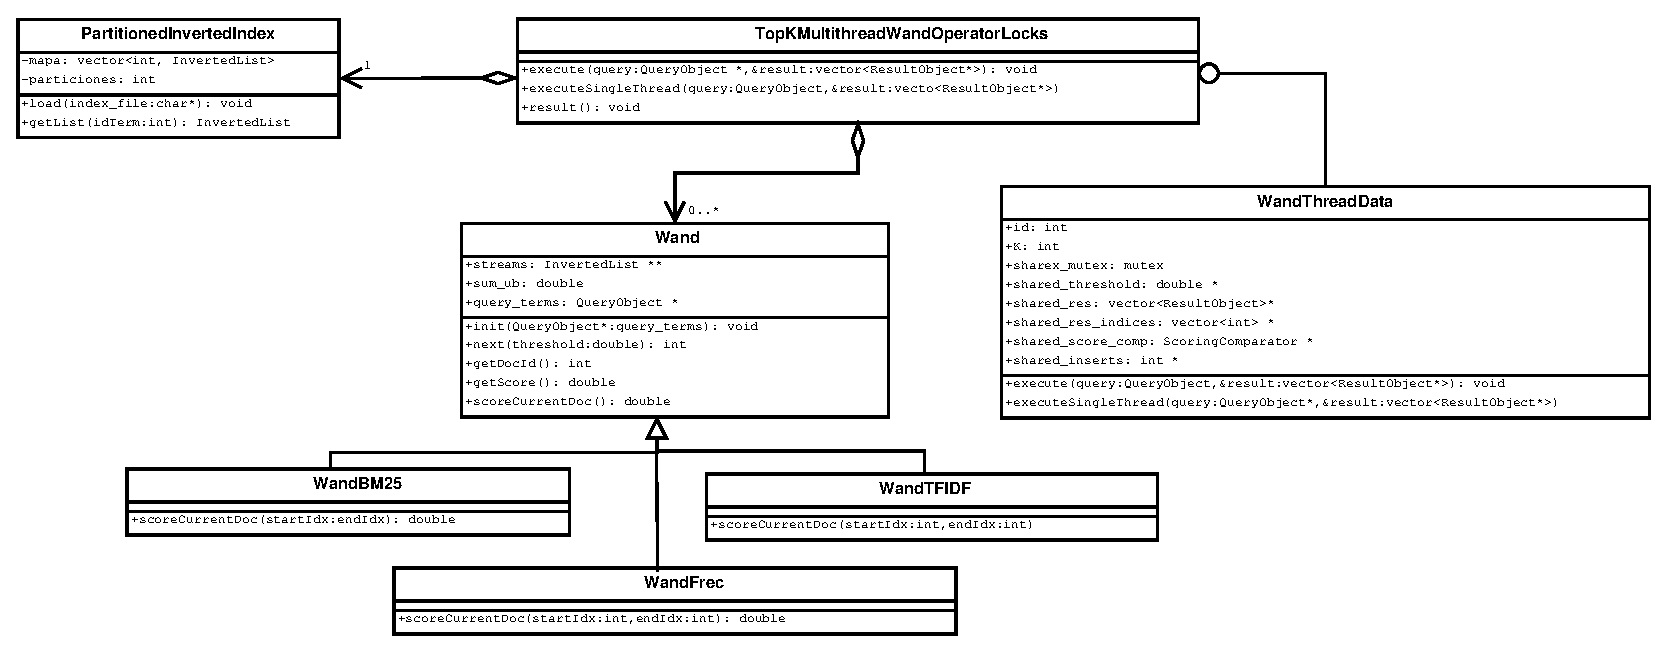
\includegraphics[scale=.75]{images/TopKMultiThreadWandOperatorLocks.eps}
\caption{Diagrama de clases para el esquema SH}
\label{fig:TopKMultiThreadWandOperatorLocks}
\end{figure}
\chapter{Métodos de predicción de rendimiento}
\label{cap:prediccion}
Lograr bajos tiempos de respuestas para transacciones de lectura es uno de los objetivos principales en el diseño de un motor de búsqueda, ya que de esta forma se le puede entregar una respuesta oportuna al usuario. Aquellas transacciones de lectura que requieren una gran cantidad de tiempo en ser resueltas degradan considerablemente la satisfacción del usuario, y es por esto que las máquinas de búsqueda están optimizadas para reducir el percentil más alto de los tiempos (también llamado \textit{tail latency}) \citep{Jeon:2014}. Paralelizar el procesamiento de cada consulta es una solución promitente para reducir el tiempo de ejecución de estas \citep{Jeon:2013, Tatikonda:2011}, lo cual es posible gracias a los modernos procesadores que existen hoy en día que poseen múltiples núcleos, en donde se puede resolver una consulta paralelizando múltiples hilos de ejecución.

Conocer de antemano la eficiencia de una transacción de lectura es una ventaja muy importante, puesto que aquellas consultas que toman una mayor cantidad de tiempo en ser resueltas se les asigna un mayor número de hilos de ejecución para resolverla, de esta manera se reduce el tiempo de procesamiento de las consultas y se cumple con la cota superior de tiempo establecida. Que un sistema como un motor de búsqueda conozca anticipadamente cuánto tardará una consulta en ser procesada, permite implementar técnicas efectivas de planificación de transacciones de lecturas, por ejemplo, en el contexto de procesamiento paralelo de consultas por lotes (\textit{batches}), se pueden crear grupos de consultas que posean similares tiempos de respuesta, así se tiende a disminuir tanto el desbalance de carga entre los procesadores como el tiempo en procesar el lote completo.

Existen trabajos en donde se estudia la correlación de algunos estadísticos presentes en las listas del índice invertido con el tiempo de respuesta de una transacción de lectura \citep{Macdonald:2012, Hauff:2010, He:2004}. El más intuitivo es el número de documentos que hay en una lista invertida, si una consulta posee términos en que sus listas invertidas son largas (muchos documentos), mayor es el tiempo que toma en ser resuelta. A continuación se presentan los métodos de predicción implementados.  

\section{Método de predicción multilineal}
\label{scheduling:glasgow}
Este método predice el tiempo de respuesta de una transacción de lectura y está basado en una regresión lineal múltiple con 42 variables independientes \citep{Macdonald:2012}. Como la respuesta a una consulta debe ser rápida, los estadísticos obtenidos desde las listas invertidas son previamente calculados en la fase de indexamiento, y en ningún caso es parte del proceso de resolución de la consulta. Los puntajes de los documentos son obtenidos mediante el método de \textit{ranking} BM25. 

Si bien es cierto que la regresión lineal posee 42 variables independientes, desde las listas invertidas se extraerán solo 14 estadísticos, ya que las 42 variables independientes se forman aplicando funciones de agregación sobre estos estadísticos. El estudio y el análisis estadístico de cada una de las variables involucradas en la regresión y su impacto en el tiempo está disponible en \citep{Macdonald:2012, Hauff:2010, He:2004}. A continuación se describe cada uno de los estadísticos $s(t)$ calculados en el proceso de indexamiento \citep{Croft:2009} de un sistema de recuperación de información.


\begin{list}{}{}
	\item \textbf{Media aritmética}. La media aritmética del puntaje de los documentos.

	\item \textbf{Media geométrica}. La media geométrica del puntaje de los documentos.

	\item \textbf{Media harmónica}.  La media harmónica del puntaje de los documentos. 

	\item \textbf{Máximo puntaje}. Se obtiene el puntaje máximo perteneciente a algún documento dentro de la lista invertida. En otras palabras, se obtiene el \textit{upper bound} $UB_t$ de la lista. 

	\item \textbf{Varianza del puntaje}. Se extrae desde a lista invertida del término $t$, la varianza del puntaje de los documentos. 
	
	\item \textbf{Número de documentos}. Largo de la lista invertida. 

	\item \textbf{Número de maximos}. Número de veces en que aparece un nuevo puntaje máximo, es decir, el número de veces en que el \textit{upper bound} es actualizado. 

	\item \textbf{Número de documentos mayor a la media}. Número de documentos con puntaje superior al puntaje promedio. 
	
	\item \textbf{Número de documentos con puntaje máximo}. Número de documentos que poseen el puntaje máximo en la lista invertida del término $t$. 
	
	\item \textbf{Número de documentos dentro del 5\% más alto}. Número de documentos cuyos puntajes están dentro del 5\% superior. 
	
	\item \textbf{Número de documentos dentro del 5\% del umbral (\textit{threshold})}. Número de documentos cuyos puntaje están dentro del 5\% superior o 5\% inferior al \textit{threshold}. Recordar que el \textit{threshold} es el puntaje más bajo dentro del conjunto de \textit{top-K}.
	
	\item \textbf{Número de inserciones en el conjunto de los mejores $K$ documentos}. Para obtener este estadístico se asume que el término $t$ es una consulta con un solo término, se resuelve esta consulta con el método Wand y se calcula el número de inserciones de documentos que se hizo al \textit{heap}. Recordar que las inserciones al \textit{heap} ocurren cuando el puntaje completo del documento, supera al \textit{threshold}.
	
	\item \textbf{Frecuencia inversa de documento del término}. Se calcula el \textit{idf} del término $t$ \citep{Baeza-Yates:2011}.
	
	\item \textbf{Tiempo en ser procesado el término}. Tiempo que toma en ser procesado el término como si fuese una consulta de un solo término.

\end{list}

Los 14 estadísticos descritos anteriormente son la base para la implementación del predictor y estos son calculados por cada término del índice invertido. Adicionalmente se definen tres funciones de agregación que se usará por cada consulta: máximo, varianza y suma. El proceso es el siguiente, para cada consulta que llega al sistema, se toman los 14 estadísticos de cada uno de los términos que la conforman, luego se aplica las funciones de agregación a los estadísticos de los términos. Por ejemplo, suponga que llega dos consultas al sistema $q_1$ y $q_2$, ambas tendrán asociada un vector de 14 estadísticos $E_{q_1}$ y $E_{q_2}$ respectivamente, las funciones de agregación para el estadísticos de la media aritmética será calculado como sigue: $e_1 = max\{E_{q_1}(0), E_{q_2}(0)\}$, $e_2 = var\{E_{q_1}(0), E_{q_2}(0)\}$, $e_3 = sum\{E_{q_1}(0), E_{q_2}(0)\}$. De esta forma, con solo el primer estadístico (la media aritmética) se obtienen tres variables independientes. Si esto se extrapola a cada estadístico, se obtienen los 42 requeridos por el método. 
La Tabla \ref{tabla:estadisticosGlasgow} muestra un resumen de lo escrito anteriormente en donde se muestra cada uno de los estadísticos y los agregadores a utilizar. 

\begin{table}[!ht]
\centering
\caption{Resumen de los estadísticos para la predicción multilineal}
\begin{tabular}{|l|}
\hline
\multicolumn{1}{|c|}{Estadísticos de términos $s(t)$} \\ \hline
1. Media aritmética \\ 
2. Media geométrica \\ 
3. Media harmónica \\ 
4. Puntaje máximo \\ 
5. Varianza del puntaje \\ 
6. Número de documentos \\ 
7. Número de máximos \\ 
8. Número docs $>$ media \\ 
9. Número docs = máximo puntaje \\ 
10. Número docs dentro del 5\% más alto \\
11. Número docs dentro del 5\% del \textit{threshold} \\ 
12. Número de inserciones al conjunto top-K \\ 
13. IDF \\ 
14. Tiempo en resolver $t$ como consulta \\ \hline
\multicolumn{1}{|c|}{Agregadores A()} \\ \hline
a. Máximo \\ 
b. Varianza  \\ 
c. Suma \\ \hline
\end{tabular}
\label{tabla:estadisticosGlasgow}
\end{table}

\section{Método de predicción neuronal}
\label{scheduling:neuronal}
Se implementa un método de predicción basado en una red neuronal \textit{backpropagation} \citep{Rumelhart:1988}. La característica de este tipo de redes es que utilizando al menos una capa oculta puede aproximar cualquier tipo de función o relación continua entre un grupo de variables de entrada y salida, debido a que utiliza un método de entrenamiento en la que se propaga el error hacia atrás, de esta forma la red neuronal va generalizando una asociación entre la entrada y salida \citep{Fausett:1994}. 

Para la implementación del modelo se utilizan las mismas 42 variables independientes del esquema anterior con dos neuronas en la capa oculta, la idea es que el tiempo que toma la predicción no genere un impacto negativo en el tiempo de procesamiento de la consulta. El objetivo es minimizar el error de la estimación de tiempo.
\chapter{Estrategias de planificación de queries}
\label{cap:planificacion}
Los motores de búsqueda verticales son sistemas dedicados a un solo propósito e ideado con el propósito de lidiar con cargas de trabajos dinámicas. Un ejemplo de un motor de búsqueda vertical es un motor de publicidad que ejecuta una consulta cada vez que un usuario abre un correo electrónico en por ejemplo, el servicio de \textit{Yahoo! mail}; de esta forma se muestra publicidad de acuerdo al contenido del correo electrónico. Eventualmente millones de usuarios concurrentes están conectados a sus correos electrónicos, por lo que la carga de trabajo esperada para el motor de búsqueda puede llegar a órdenes de las cien mil consultas por segundo \citep{Gil-Costa:2013}. Adicionalmente, el hecho que las actualizaciones en un motor de búsqueda vertical ocurran con mayor frecuencia que en uno de propósito general, hace que el diseño de los algoritmos para procesar las \textit{queries} sea diferente; también se debe permitir la actualización del índice invertido.

Por lo anteriormente mencionado, se hace imperioso tener un sistema diseñado que soporte altas cargas de trabajo, y las respuestas a consultas esten en una cota de tiempo aceptable para el usuario sin mermar la calidad de los resultados obtenidos. También es necesario que las estructuras de datos y los algoritmos implementados soporten la concurrencia entre las transacciones de lecturas y escrituras; dicho de otra forma, eventualmente el motor de búsqueda tendrá que dejar de procesar consultas para poder servir las transacciones de escritura que actualizan el índice invertido.

A continuación se muestra las diferentes estrategias de planificación de transacciones de lectura abordadas en el presente trabajo utilizando diferentes enfoques; se presentan tres enfoques diferentes: El primero consiste en crear bloques de consultas en donde previamente a cada una de ellas se le asigna el número de hebras que utilizará en su resolución, luego el bloque es procesado en paralelo por los diferentes hilos de ejecución asignados; El segundo enfoque corresponde a unidades de trabajos, en la que a cada \textit{query} se le asigna un número determinado de unidades de trabajo y los \textit{threads} compiten por ellas desde una cola; (3) El tercer enfoque y último es el más básico, cada hilo de ejecución se hace cargo de una consulta y lleva a cabo su procesamiento, en este enfoque la competencia entre los hilos de ejecución es por las consultas. 


\section{Estrategias por bloques}
\label{scheduling:bloques}
Un sistema de planificación de un motor de búsqueda trabaja en un contexto \textit{online}, esto significa que desconoce las transacciones que vendrán en el futuro y que cuando llega una nueva transacción de lectura, se debe tomar una decisión rápida acerca de qué hacer con ella. En el contexto del presente trabajo, para que el planificador tome una decisión se debe conocer el número de hebras con los que cada \textit{query} será resuelta y para lo cual se utiliza los predictores mostrados en \ref{cap:prediccion}; una vez que se predice el tiempo, se asigna el numero de hilos de ejecución con los que la consulta será resuelta para cumplir con la cota de tiempo impuesta.  

Bajo el contexto de un motor de búsqueda en el que se debe planificar transacciones de lecturas que eventualmente serán resueltas de forma paralela por diferentes hilos de ejecución, existe una estrategia teórica llamada FR que aborda este problema \citep{Ye:2007} y se adapta a nuestro escenario de un motor de búsqueda vertical; además se propone dos nuevas estrategias siguiendo el mismo enfoque de FR, pero estas enfocadas principalmente en mejorar la asignación de consultas a bloques, para así reducir el tiempo ocioso de las hebras. 

\subsection{Estrategia FR}
\label{scheduling:fr}
La estrategia de planificación FR asume que cada query que llega al motor de búsqueda posee el tiempo en que se domorará en ser procesada. 
Sehace una clsificación de las queries entre Big y Small con el objetivo de crear estructuras de datos denominadas Rooms y Walls, en donde Walls y Tooms estarán formadas por queries Bigs y Smalls respectivamente. Ambas estructuras tienen un número máximo de máquinas disponibles para procesar las queries. Una consulta es Big si el número de máquinas requeridas para procesarlas es m (siendo m el número de máquinas disponibles),, de lo contrario, la query es small. 
% Debe estar bloqueada porque eventualmente el ejecutador de queries estará sacando

% ----  Descripción del algoritmo ----
Como se puede ver en el Algoritmo \ref{alg:fr}, cuando una nueva query llega al sistema se analiza si esta es de tipo Big o Small; esto se hace en el método isBig(), que retorna verdadero si es que el número de máquinas requeridas para procesarla es igual al máximo de máquinas disponibles, de lo contrario retorna falso. Si la consulta es big, entonces se crea un nuevo Wall, se agrega la query al bloque y el bloque es planificado en la lista de planificación SchedulingList. Si se está en presencia de una transacción de lectura Small, entonces se busca algún bloque disponible para planificar la query, esto se hace desde el primer bloque abierto para recibir transacciones de lectura hasta el final de la schedulingList. Finalmente, si es eventualmente no se encuentra algún bloque disponible para planificar la query, entonces se crea un nuevo bloque Room, se asigna la consulta al bloque y se asigna el bloque a la lista de scheduling. Cabe destacar que se dice que un bloque está abierto cuando (isOpen) cuando aún le quedan máquinas disponibles o cuando el proceso de ejecución ya ha tomado las queries de este bloque para resolverlas.
%----- Fin descripción algoritmo ----

\begin{algorithm}[!th]
\caption{\em $schedulerFR::assignQuery(L, Q)$: Planificación de consulta estrategia FR}
\label{alg:fr}
\begin{algorithmic}[1]
\REQUIRE Una SchedulingList $L$ en donde se hará la planificación, QueryObject $Q$ a planificar
\ENSURE SchedulingList $L$ con la nueva query planificada

\IF {$isBig(query)$}
	\STATE $block = new Wall();$
	\STATE $block \rightarrow addQuery(query);$
	\STATE $L \rightarrow addBlock(block);$
\ELSE
	\STATE $asignada = false;$
	\FOR {$ i = L \rightarrow firstOpenBlockLocked()...L \rightarrow sizeLocked()$}
		\STATE $room\_block = L \rightarrow getBlockLocked(i);$
		
		\IF {$(room\_block \rightarrow isOpen()) AND 
				(room\_block \rightarrow freeThreads() >= query \rightarrow getThreads())$
			}
			\STATE $room\_block \rightarrow addQuery(query)$
			\STATE $asignada = true$
			\STATE $break;$
		\ENDIF
	\ENDFOR
	
	\IF {$!(asignada)$}
		\STATE $block = new Room();$
		\STATE $block \rightarrow addQuery(query);$
		\STATE $L \rightarrow addBlockLocked(block);$		
	\ENDIF
\ENDIF

\end{algorithmic}
\end{algorithm}


// Esquema de ejecución

// Algoritmo

// Ejemplo de cómo van quedando los bloques

Se intuye que habrá pérdida de eficiencia al final de cada bloque. 


\subsection{Estrategia Times}
\label{scheduling:times}
La idea de esta estrategia es separar las queries que tengan tiempos de procesamiento muy diferentes, es decir, se crearán bloques de queries que tienen poca diferencia de tiempo, de esta forma se quiere reducir el tiempo perdido entre un bloque y otro. Cada bloque b tendrá un tiempo t, que será el menor tiempo perteneciente a alguna de las consultas ya planificadas en el bloque. La métrica establecida para que una query sea planificada en un bloque, es que el tiempo del bloque tb no puedo doblar al tiempo de la consulta tq, y viceversa. Si esta condición falla, entonces significa que la query q que se está intentando planificar posee tiempos que se escapa a los rangos de tiempo del bloque b. A continuación se muestra el algoritmo para la presente estrategia

\begin{algorithm}[!th]
\caption{\em $schedulerTimes::assignQuery(L, Q)$: Planificación de consulta estrategias Times}
\label{alg:times}
\begin{algorithmic}[1]
\REQUIRE Una SchedulingList $L$ en donde se hará la planificación, QueryObject $Q$ a planificar
\ENSURE SchedulingList $L$ con la nueva query planificada
	\STATE $blocks_viewed = 0$
	
	\FOR {$ i = L \rightarrow firstOpenBlockLocked()...L \rightarrow sizeLocked()$}
		\STATE $block = lista\_bloques \rightarrow getBlockLocked(i);$
		
		\IF {$block \rightarrow isOpen() AND block \rightarrow freeThreads() \geq query \rightarrow getThreads()$}
			\STATE $queries = block \rightarrow getQueries();$
			\STATE $tiempo\_min = queries[0] \rightarrow getEstimatedTime();$
			
			\FOR {$ j = 1 ...queries->size()$}
				\IF {$queries[j] \rightarrow getEstimatedTime() < tiempo_min$}
					\STATE $tiempo\_min = queries[j] \rightarrow getEstimatedTime();$
				\ENDIF
			\ENDFOR
			
			\IF {$tiempo\_min < estimated\_time$}
				\STATE $diff = 2*tiempo_min - estimated_time;$
			\ELSE
				\STATE $diff = 2*estimated_time - tiempo_min;$
			\ENDIF
			
			\IF {$diff < 0$}
				\STATE $diff = 0.0-diff;$
				\IF {$diff < best_diff$}
					\STATE $best_diff = diff;$
					\STATE $best_block = i;$
				\ENDIF
			\ELSE
				\STATE $valido = true;$
			\ENDIF
			
			\IF {$ valido $}
				\STATE $block \rightarrow addQuery(query);$
				\STATE $asignada = true;$
				\STATE $break;$
			\ENDIF
			
			\STATE $bloques_revisados++;$
			
			\IF {$bloques_revisados \geq max_bloques_rev$}
				\STATE $break;$
			\ENDIF
			
		\ENDIF
		
	\ENDFOR
	
	\IF {$ ! asignada $}
		\IF {$ (bloques\_revisados \geq max\_bloques_rev) $}
			\STATE $block = lista\_bloques \rightarrow getBlockLocked(best\_block);$
			\STATE $block \rightarrow addQuery(query);$
		\ELSE
			\STATE $block = new QueryBlock();$
			\STATE $block \rightarrow addQuery(query);$
			\STATE $lista\_bloques \rightarrow addBlockLocked(block);$
			
		\ENDIF	
	\ENDIF

\end{algorithmic}
\end{algorithm}




\subsection{Estrategia TimesRanges}
\label{scheduling:fr}


\section{Estrategia unidades de trabajo}
\label{scheduling:unidadestrabajo}
Decir que aquí para planificar se necesita conocer las unidades de trabajos requeridas en vez de threads como en las estrategias por bloques.

Con respecto a los esquemas explicados hasta ahora, el esquema 1TQ tiene la ventaja que no solo requiere menos control, sino que también permite a los hilos de ejecución trabajar sin pausa mientras un \textit{batch} de consultas está siendo procesado. En esta sección se propone un esquema híbrido basado en unidades de procesamiento (\textit{Processing Units}) que aproveche las ventajas de ambos enfoques. (se requiere ver el tema de bloques).
En este nuevo esquema de planificación, las consultas pasan a través de una fase en la cual cada \textit{query} es evaluada y se determina un apropiado número de unidades de procesamiento (\textit{processing units}) para poder resolver dicha consulta. Este proceso es llevado a cabo de manera similar al proceso en donde se determina la cantidad de \textit{threads} apropiados para resolver una determina transacción de lectura. Este número de unidades de procesamiento es creado y asociado a cada consulta, finalmente se guarda en una cola de unidades de trabajo. Un conjunto de \textit{threads} consumidores extraen las unidades desde la cola y las procesa independientemente. Cuando un \textit{thread} finalice el procesamiento de la unidad de trabajo actual automáticamente leerá la siguiente unidad de trabajo desde la cola. 
Generalmente lo que se hace habitualmente es estimar el número de \textit{threads} con el que se resolverá la consulta, como se muestra en la Figura \ref{fig:unit_process} en este nuevo enfoque se intenta estimar el número de unidades de trabajo con el que se resolverá cada consulta. Además, se debe controlar el acceso concurrente de los hilos de ejecución a la cola de unidades de trabajo, de tal manera que solo un thread tenga acceso exclusivo a la estructura de datos. 

\begin{figure}[!th]
\centering
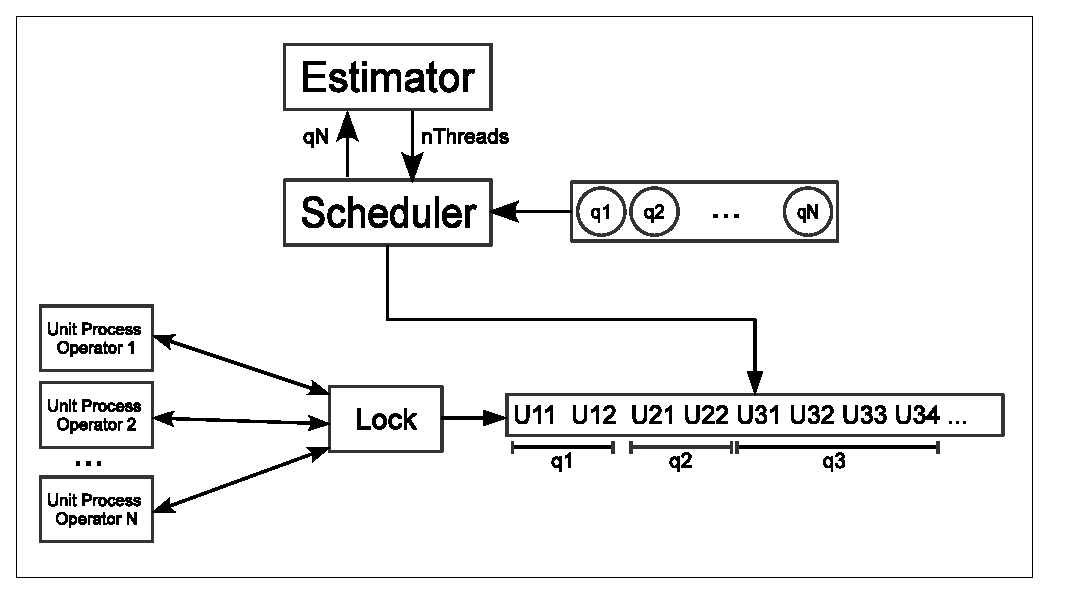
\includegraphics[scale=.75]{images/unit_process.eps}
\caption{Procesamiento de consultas utilizando unidades de trabajo}
\label{fig:unit_process}
\end{figure}

El procesamiento de cada hilo de ejecución es una versión de Wand con heap compartido (SH), adaptado de manera tal que cada unidad de trabajo es resuelta independientemente de si existen otras unidades siendo procesada al mismo tiempo o no. La única excepción es que la unidad que inicializa la consulta es siempre ejecutada antes del resto de las otras unidades de la misma consulta y la entrega de resultados se hace una vez que todas las unidades de trabajo de la \textit{query} han finalizado. Este enfoque híbrido permite reducir el tiempo perdido al final de cada \textit{batch} sin generar una importante pérdida de trabajo mientras las \textit{queries} del \textit{batch} están siendo procesadas.



\section{Estrategia \textit{1TQ}}
\label{scheduling:baseline}
Un simple camino para construir un sistema que responda a múltiples consultas simultáneamente usando múltiple hilos de ejecución, es usando estos hilos de manera independiente. Para hacer esto se debe mantener un conjunto de \textit{threads} consumidores que trabajarán en paralelo y se encargarán de resolver las \textit{queries} secuencialmente (una a una) desde una misma cola, esto es lo que en este trabajo se denomina estrategia de Un Thread Por Query (1TQ). En la Figura \ref{fig:1TQ} se puede apreciar el esquema de ejecución en donde cada uno de los procesos genera una petición de alguna consulta en la cola, si quedan \textit{queries} por procesar entonces se le asigna al proceso una consulta que tendrá que resolver de manera secuencial. Se debe tener en cuenta que cada vez que un proceso genera una solicitud de \textit{query}, se bloquea la estructura de datos que contiene las consultas a procesar y luego se procesa la solicitud, de esta forma se asegura un acceso seguro por parte de los distintos \textit{threads}. 

\begin{figure}[H]
\centering
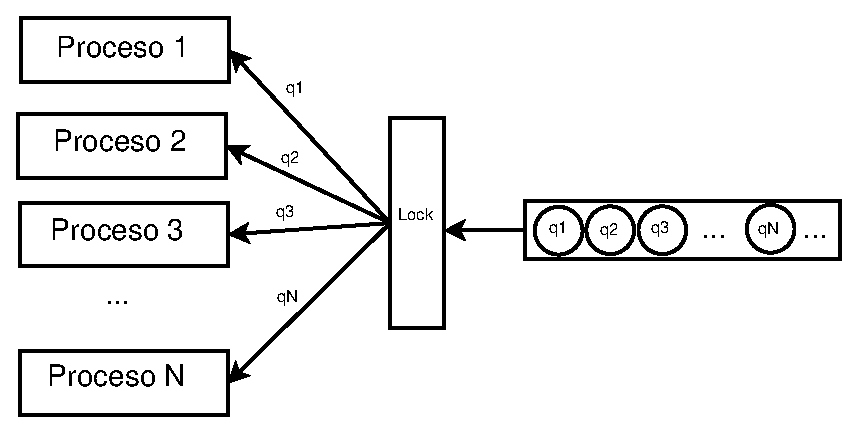
\includegraphics[scale=.75]{images/1TQ.eps}
\caption{Ejemplo de procesamiento estrategia 1TQ}
\label{fig:1TQ}
\end{figure}

Este esquema tiene la ventaja que es simple y fácil de implementar y controlar. Sin embargo, existen sistemas de recuperación de la información como los motores de búsqueda verticales que cuando están ejecutando \textit{batches} de \textit{queries} deben parar su ejecución porque transacciones de escritura han llegado al sistema, y este deben actualizar la información del índice invertido. Solo después de la fase de actualización el sistema es capaz de ejecutar el siguiente \textit{batch} de transacciones de lectura. Al final de cada conjunto de consultas, es posible que algunos hilos de ejecución del sistema finalicen su trabajo y que no tengan más \textit{queries} para procesar, por lo que ellos tienen que esperar que los \textit{threads} restantes finalicen su trabajo antes que el sistema entre en la fase de actualización de su índice invertido o bien, se pase a la ejecución del siguiente \textit{batch} de consultas.
Sin embargo, aunque cada hilo de ejecución está secuencialmente ejecutando una transacción de lectura diferente, algunas de estas operaciones puede tomar un tiempo cosiderable, de esta forma se produce una importante pérdida de eficiencia, aunque la intuición nos dice que esto se puede mitigar con \textit{queries} que requieran poca cantidad de tiempo para ser procesada (trabajos pequeños o \textit{small jobs}). 
En la Figura \ref{fig:small_jobs} queda reflejado lo dicho en el párrafo anterior. Si los trabajos que cada \textit{thread} está ejecutando son pequeños, entonces probablemente la pérdida de trabajo al final de cada \textit{batch} de consultas será menor al trabajo que se pierde cuando los trabajos son grandes (ver Figura \ref{fig:large_jobs}).  


\begin{figure}[H]
\centering
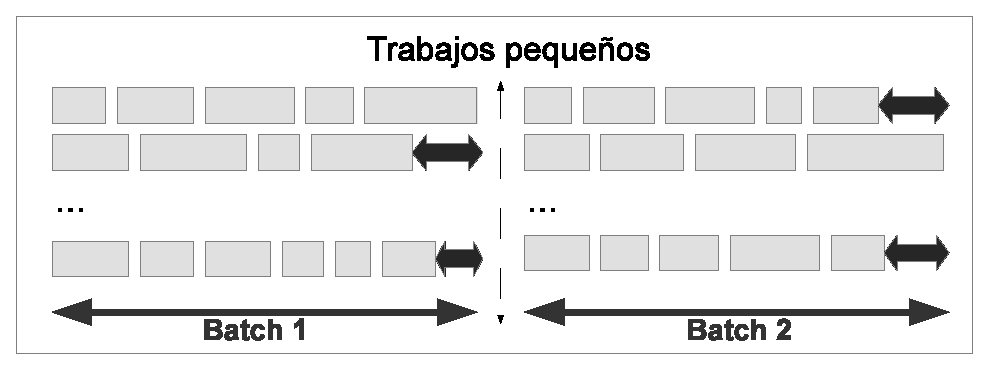
\includegraphics[scale=.75]{images/small_jobs.eps}
\caption{Ejecución en paralelo de \textit{small jobs}}
\label{fig:small_jobs}
\end{figure}

\begin{figure}[H]
\centering
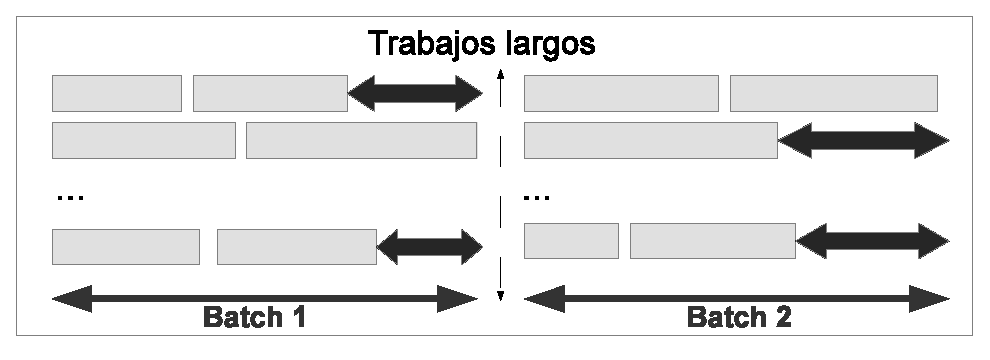
\includegraphics[scale=.75]{images/large_jobs.eps}
\caption{Ejecución en paralelo de \textit{large jobs}}
\label{fig:large_jobs}
\end{figure}
\chapter{Evaluación experimental}
\label{cap:evaluacionexperimental}

En el presente capítulo se presenta los resultados obtenidos de las diferentes implementaciones para los métodos propuestos en la secciones anteriores. Se comienza por la implementación de los diferentes enfoques de los métodos de procesamiento de transacciones de lectura, posteriormente se muestra los resultados obtenidos para los diferentes métodos de predicción de tiempos de respuestas para consultas y el comportamiento que tienen para diferente conjunto de datos. Finalmente se presenta el comportamiento de las diferentes estrategias de planificación presentadas para diferentes tipos de escenarios.


\section{Hardware y conjunto de datos}
\label{evaluacionexperimental:hardwareydatos}
%% Hablar un poco del hardware utilizado en los experimentos

Se utilizaron dos conjuntos de datos para llevar a cabo los experimentos, estos son frecuentemente usados por la comunidad del área de Information Retrieval para experimentar. El primero de ellos es GOV2, este conjunto es una colección de aproximadamente 25 millones de páginas Web obtenida desde los dominios .gov y que pesa 426 GB. La otra colección de datos utilizada es la ClueWeb09, la cual fue creada para apoyar la investigación en recuperación de la información y las tecnologías relacioanadas con el lenguaje humano. Consiste en alrededor de un billón de páginas en diez lenguajes diferentes y 50 millones en Inglés. ClueWeb09 pesa 5 TB en forma comprimidad y 25 TB descomprimida. 

% Las consultas (queries)



\section{Wand multithreaded}
\label{evaluacionexperimental:wm}
En esta sección se muestra la implementación de dos enfoques para el procesamiento de consultas a través del algoritmo Wand \citep{Broder:2003}. El primer enfoque es el esquema de heap locales (LH), en el que cada thread obtiene sus mejores documentos para una query dada y luego una hebra maestra se encarga de mezclar todos los resultados de cada uno de los threads para construir en conjunto top-K final; el segundo enfoque es el enfoque de heap compartido (SH), en el que se tiene un heap visible a todos lo shilos de ejecución y en donde ellos compiten por el acceso a esta estructura de datos. El detalle del diseño de los enfoques LH y SH están disponibles en \ref{scheduling:wlh} y \ref{scheduling:whc}. 

\subsection{Esquema LH}
\label{evaluacionexperimental:esquemalh}

\begin{figure}[th!]
\centering
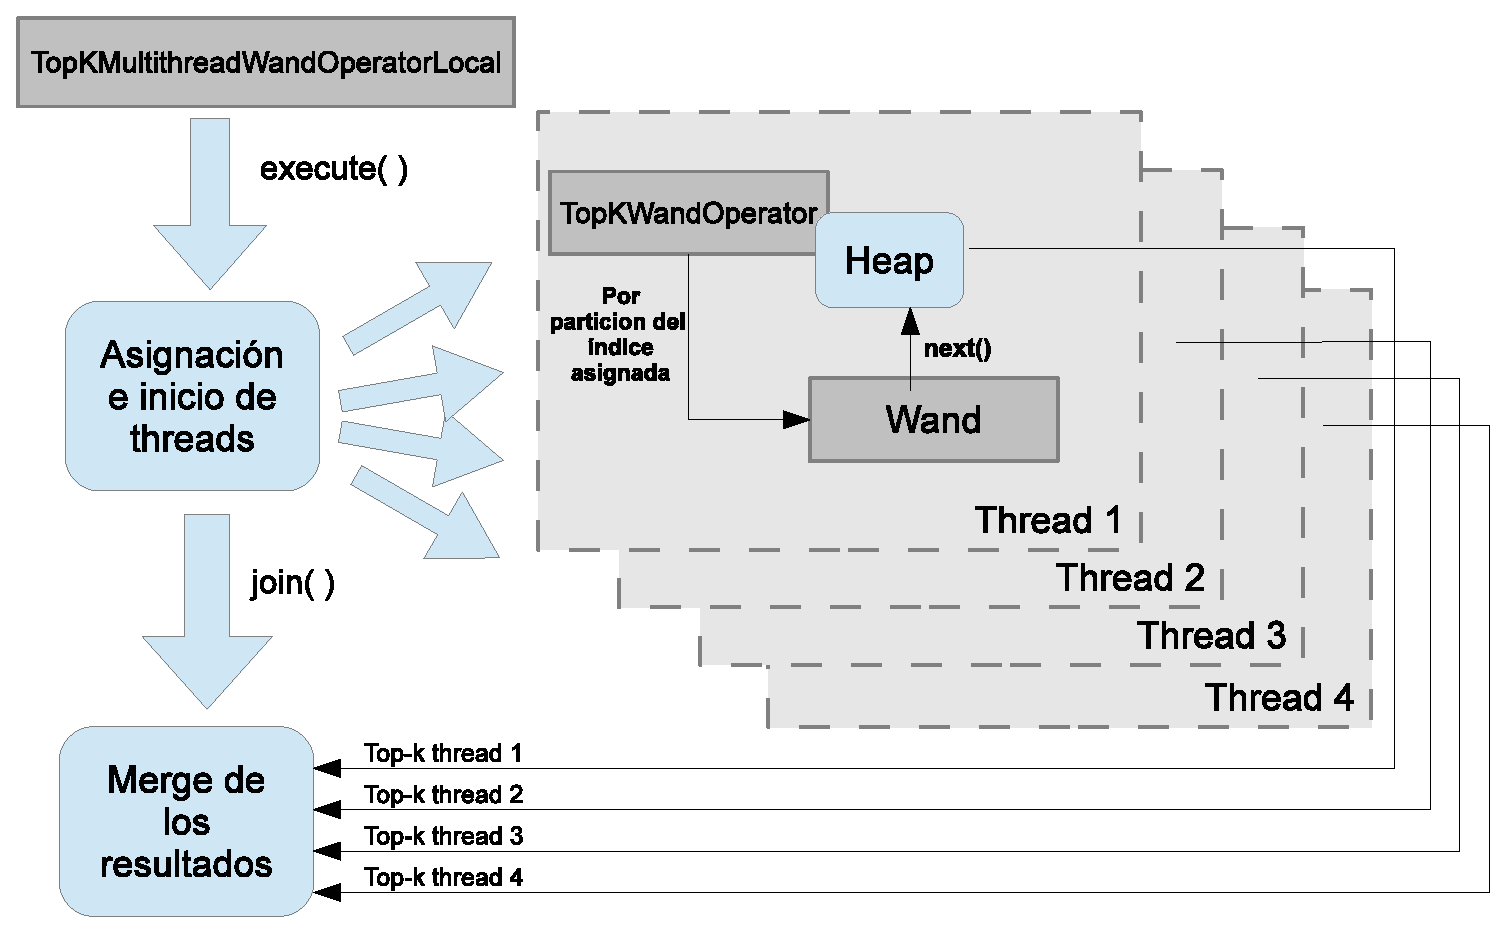
\includegraphics[scale=.75]{images/ejecucion_topkmultithreadwandopLOCAL.eps}
\caption{Esquema de ejecución enfoque LH}
\label{fig:esquema_ejecucion_wandlh}
\end{figure}



\subsection{Esquema SH}
\label{evaluacionexperimental:esquemash}

\begin{figure}[th!]
\centering
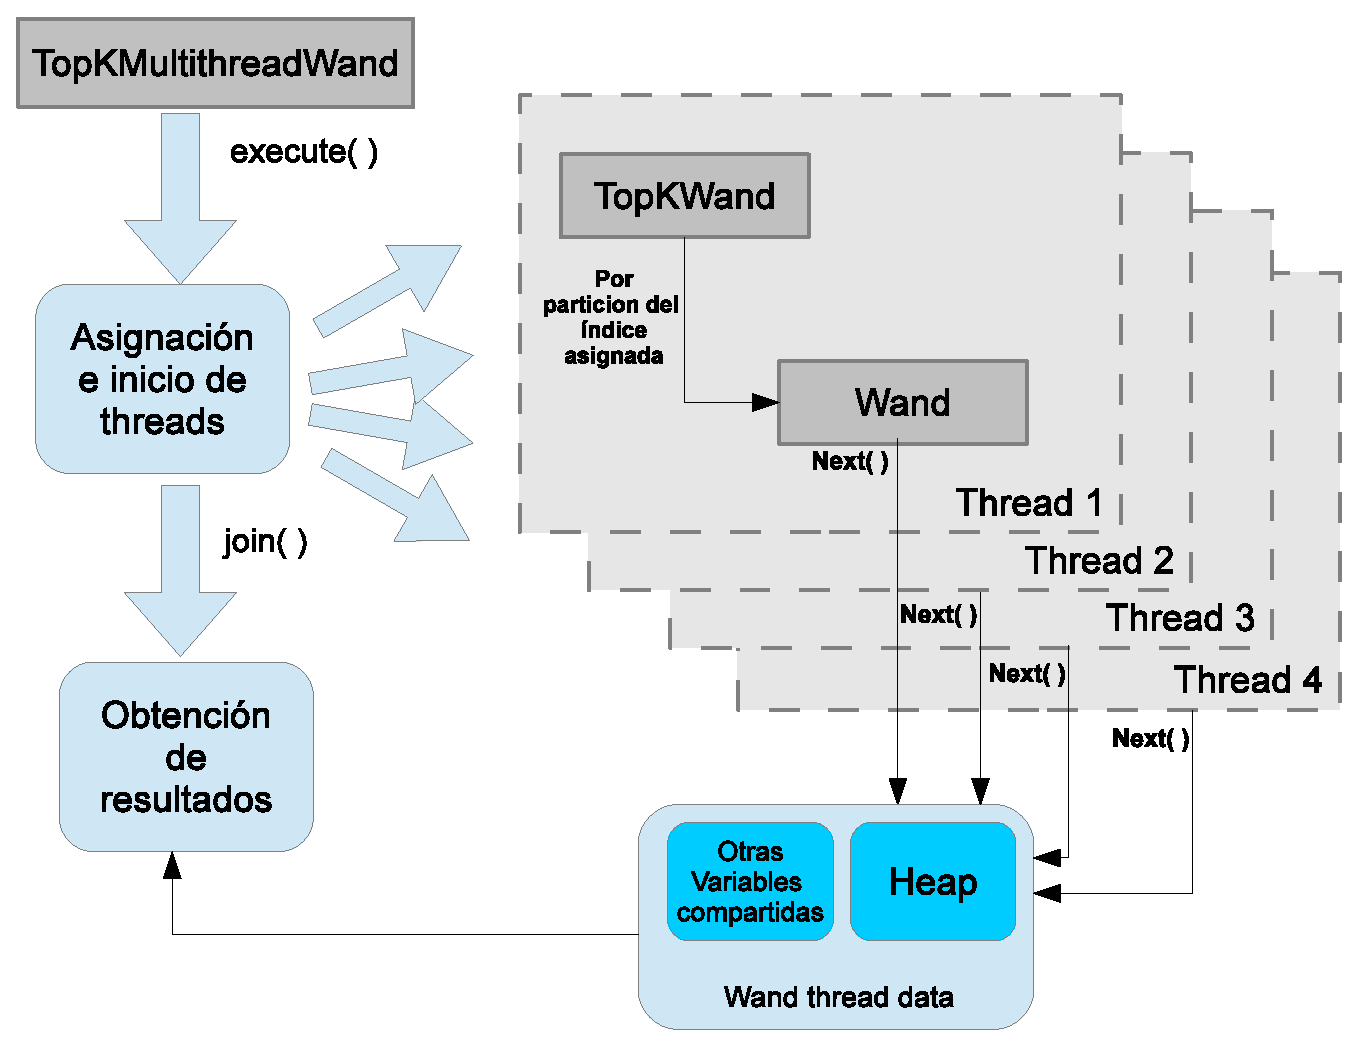
\includegraphics[scale=.75]{images/ejecucion_topkmultithreadwandopCOMPARTIDO.eps}
\caption{Esquema de ejecución enfoque SH}
\label{fig:esquema_ejecucion_wandsh}
\end{figure}












\begin{comment}

// Cómo se llevaron a cabo los experimentos
// Datos
// Máquina
// Programación 


Recordar que en el esquema Wand LH cada uno de los hilos de ejecución computa el conjunto top-K local y luego la hebra maestra hace la mezcla de resultados escogiendo el mejor conjunto top-K global. Este enfoque tiene la ventaja de que es simple de implementar, puesto que no se requiere mecanismos para controlar el paralelismo entre los threads. Sin embargo, se requiere que cada uno de los (P - 1) threads envíe su conjunto solución a la hebra maestra (que también computó su propio conjunto solución), para que crear el resultado final de entre los P x K documentos, donde P es el número de threads encargadas de resolver la consulta y K se es el tamaño del conjunto que se quiere obtener. 

Los resultados en \citep{Rojas:2013} muestran indicios que el esquema LH tendría ventajas por sobre el SH para aquellas transacciones que toman poco tiempo en ser resueltas. 

El Código \ref{code:topkmultithreadwandoperatorlocal} muestra la implementación de la clase que está encargada de llevar a cabo la lógica en la ejecución del enfoque Wand LH. El método execute es el encargado de llegar a cabo la resolución de la consulta, recibe como entrada la query a ser resuelta y un vector de resultados; adicionalmente, este método es el encargado de lanzar los threads con que se resolverá cada consulta y a cada uno de ellos le asiga un objeto de tipo TopKWandOperator (arrops), para obtener los resultados y escribirlos en el vector results. Todo este proceso es llevado a cabo usando el tamaño del conjunto que se quiere obtener (k) y además el índice invertido (indice).


\begin{figure}[!th]
\centering
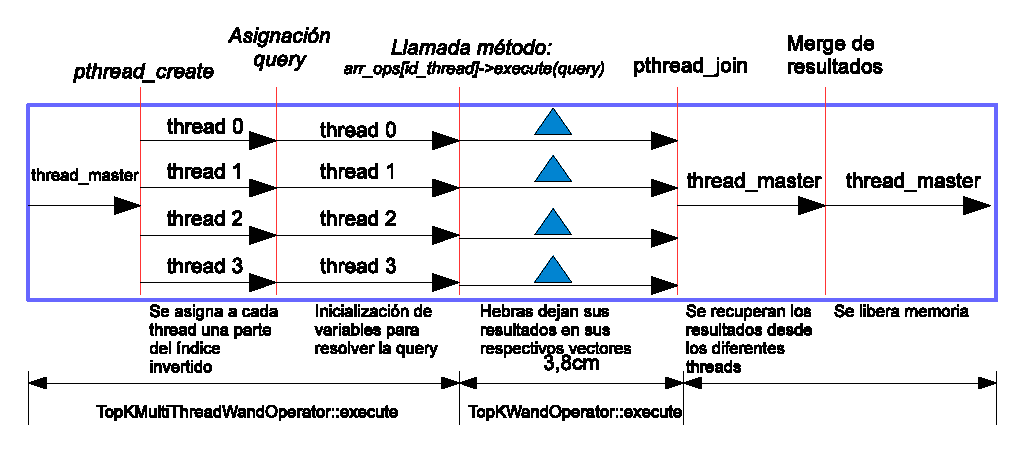
\includegraphics[scale=.75]{images/ejecucion_wandlh.eps}
\caption{Ejemplo de ejecución esquema Wand LH}
\label{fig:ejecucion_wandlh}
\end{figure}

  

%El hecho que en el esquema de heap locales no se requiere mecanismos de control de paralelismo en su implementación, posee ventajas para queries cortas en su procesamiento 
%Figura




\lstinputlisting[label=code:topkmultithreadwandoperatorlocal, caption=Implementación de la clase TopKMultithreadWandOperatorLocal.h, language=C++]{code/TopKMultithreadWandOperatorLocal.h}

Mostrar topK Wand operator

\end{comment}



\begin{comment}

el proceso de descarte tiende a ser más eficiente porque los documentos con mayor puntaje tienden a estar en el heap

Se habla un poco de las ventajas que se tenía con este esquema nuevamente, qué se hizo para la implementación, cómo se programó, etc. 

Se muestra el código y ojalá se muestra algún flujo de ejecución para una query específica.

%\lstinputlisting[language=C++]{code/TopKMultithreadWandOperatorLocal.h}

Se muestra un gráfico y tabla de eficiencia.

\end{comment}

\subsection{Resultados obtenidos}
\label{evaluacionexperimental:resultadosObtenidos}

En la Figura \ref{fig:tiempos_wand} se puede observar el tiempo promedio del enfoque LH y el enfoque SH en resolver un conjunto de 10000 consultas de la colección gov2. A medida que crece el número de threads, el enfoque de heaps compartidos toma ventaja por sobre el enfoque de heaps locales, sin embargo, con un thread se puede observar que LH (117.486 ms) requiere un tiempo menor que SH (130.591 ms), esto se debe porque aquí no se usa una estructura de dato compartida que retrase a los hilos de ejecución esperando a que otros la liberen. LH requiere menos tiempo en resolver el log de consultas para 2,4,8 y 16 threads. 

El esquema LH puede estar muy supeditado a la distribución de documentos en las listas del índice invertido, ya que si un thread procesa su parte corrrespondiente del índice invertido en donde los mejores puntajes se encuentran al final, entonces el heap tendrá un umbral bajo el proceso de descarte omitirá pocos documentos, esto implca que el tiempo de ejecución requerido será mayor, retrasando el proceso que mezcla los resultados para obtener el conjunto top-K dinal. 

Como el esquema SH ocupa un solo heap para obtener el conjunto top-K final, el heap tiende a llenarse rápidamente con los mejores documentos globales, esto implica que el puntaje mínimo del heap (que trabaja de umbral) tiende a crecer rápidamente, permitiendo un mejor descarte de documentos y menos tiempo de ejecución para las hebras. 

Adicionalmente en la Figura \ref{fig:eficiencias_wand} se puede ver que en forma general con la estrategia de enfoques compartidos se obtiene mejores eficiencias que con la estrategia LH. En Con SH la mejor eficiencia que se obtiene es con 4 threads (0.962 ms), mientras que con 2 y con 8 threads se obtiene una eficiencia de 0.887 y 0.8312600071 milisegundos; en general se obtiene buenas eficiencias para 1,2,4 y 8 hebras, sin embargo, con 16 threads la eficiencia baja considerablemente (0.5403329185) con respecto a las anteriores, esto se debe principalmente a la tecnología hyperthreading de la máquina utilizada y que el uso exclusivo del heap compartido por parte de los threads no tiene un fuerte impacto en el rendimiento.  
La eficiencia baja de LH se debe porque para obtener el conjunto top-K final de una consulta debe haber una sincronización de todos los threads en que cada uno de ellos envíe sus top-K locales a la hebra maestra y además porque existe un costo adicional de calcular el conjunto top-K final entre los P * K documentos seleccionados (siendo P el número de procesadores). 
                     
Para los siguientes experimentos del presente trabajo se ocupará el enfoque SH para resolver las transacciones de lectura.


\begin{figure}[!ht]
\centering
\includegraphics[scale=.75]{images/tiempos_wand.eps}
\caption{Tiempos promedios de las consultas}
\label{fig:tiempos_wand}
\end{figure}

\begin{figure}[!ht]
\centering
\includegraphics[scale=.75]{images/eficiencias_wand.eps}
\caption{Eficiencias para Wand con heaps compartido y locales}
\label{fig:eficiencias_wand}
\end{figure}


\begin{comment}

Se hace una introducción.

\section{Predicción de tiempo de respuesta a transacción de lectura}
\label{evaluacionexperimental:ptrq}
Se hace experimentos con predictor perfecto

Nosotros optamos por un enfoque de Wand Heap Compartido para ser usado en los experimentos.

Se hace una breve introducción al cpaítulo anterior. 

Se menciona los resultados obtenidos con la regresión, se dice que no se tuvieron muy buenos resultados con la regresión, se deja a ver por qué no se obtuvieron muy buenos resultados (índice con los que se hicieron experimentos, consultas, etc.).

	//menos que 10% tpo esperado, menos que 25%, menos que 50% y el resto (en el timesRanges)
\subsection{Predictor perfecto}
\label{evaluacionexperimental:predictorperfecto}

Decir que no es el foco de esta tesi, que los resultados obtenidos no fueron muy buenos s y que para evaluar los algoritmos de scheduling  también se usará un predictor perfecto. Decir cómo se obtuvo un predictor perfecto y ojalá mostrar algún algoritmo.





\section{Estrategias de scheduling}
\label{evaluacionexperimental:estrategiasscheduling}

Hablar separado cada una de ellas, mostrando implementación y cómo se llevaron a cabo los experimentos.

1. Comparar las tres estrategias de scheduling (decir que TimesRanges es mejor) ==> Con predictor perfecto también?
2. Comparar TimesRanges con baseline ==> Con Predictor perfecto también.  
4. Decir los problemas que existen en cada una de las estrategias que se pierden tiempos.
3. Sacar a la luz la nueva unidades de trabajo ==> Predictor perfecto también.
4. Comparación unidades de trabajo - baseline - TimesRanges.

Conclusiones para cada uno de los gráficos realizados. 

Se intuye que habrá pérdida de eficiencia al final de cada bloque en FR.

\end{comment}
\chapter{Conclusiones}
\label{cap:conclu}
% Intro general
% Capítulo de Wand multithreading
% Conclusión 
% Capítulo de predicción de tiempos
% Conclusión
% Capítulo de estrategias de planificación
% Conclusión
% Conclusión objetivos específicos
% Conclusión general
% Aportes al área
% Trabajo futuro
Por medio del presente trabajo se ha llevado a cabo un estudio del procesamiento y planificación de transacciones de lectura que llegan a un motor de búsqueda haciendo uso de una máquina multinúcleo, en el que se adaptaron diferentes estrategias de planificación del estado del arte al contexto de un motor de búsqueda, y se evaluaron los rendimientos de cada una de ellas mediante el procesamiento de consultas por lotes. Adicionalmente se propone una estrategia de procesamiento de consultas basada en unidades de trabajo, en el que cada consulta es dividida en unidades de procesamiento y los diferentes hilos de ejecución compiten por procesar cada unidad.

El sistema implementado para resolver una transacción de lectura que llega al sistema, es flexible a hacer uso de diferentes números de hilos de ejecución; esta capacidad se logra debido a que se implementó dos versiones paralelas del algoritmo Wand, la primera es una versión con \textit{heaps} locales y la otra hace uso de un solo \textit{heap} compartido. Los resultados arrojan que utilizando la muestra de la Web Gov2 y obteniendo el conjunto de los \textit{top-100} mejores documentos, el enfoque con \textit{heap} compartido posee mejor rendimiento. 
% BMW

Con respecto a los predictores de rendimiento de transacciones de lectura, el método ML basado en una regresión lineal múltiple obtiene mejor rendimiento en la predicción que el método RN basado en redes neuronales, esto utilizando el mismo conjunto de 42 descriptores para ambos métodos. Lo mencionado anteriormente no descarta que exista una mejor solución para el método RN que incluso pueda mejorar en rendimiento al método ML, para esto se debe hacer una mejor clasificación de descriptores utilizados para la creación del modelo.
 
Las estrategias de planificación por bloques no poseen un buen rendimiento cuando el objetivo es procesar grandes cantidades de transacciones de lectura por lotes, debido a la pérdida de tiempo que existe entre la sincronización de bloques. Por otro lado, la estrategia de procesamiento de consultas por unidades de trabajo parece ser la mejor forma de reducir el tiempo total de procesar grandes cantidades de consultas por lotes y al mismo tiempo asegurar una cota superior de tiempo para cada una de ellas.

En condiciones ideales de predicciones de tiempo, la estrategia de unidades de trabajo posee mejor rendimiento que la estrategia 1TQ creada como \textit{baseline}. A medida que el tamaño de los lotes crece, la diferencia de rendimiento es menor, debido a que existen menos sincronizaciones entre lotes, lo que implica una menor pérdida de eficiencia para la estrategia 1TQ.

En el presente contexto de procesamiento de transacciones de lectura en una máquina multicore, probablemente sea una mejor idea enfocar esfuerzos en crear un predictor más simple y preciso que los vistos en el presente trabajo por sobre intentar reordenar las consultas, de esta manera se obtendrán mejores tiempos para el procesamiento del conjunto completo de consultas.

Finalmente es posible afirmar que se ha cumplido con todos los objetivos planteados al comienzo de este trabajo. Se ha desarrollado dos algoritmos de procesamiento de transacciones de lectura basados en el algoritmo Wand, una con \textit{heap} compartido y otra con \textit{heaps} locales. Se han creado estrategias de planificación \textit{online} que reordenan y adaptan dinámicamente las consultas al tamaño de las estructuras de datos disponibles; estas estrategias fueron adaptadas al contexto de un motor de búsqueda vertical en el que se procesan transacciones de lectura por lotes. Finalmente la evaluación para los métodos de predicción se hizo mediante la medición del RMSE y error relativo porcentual promedio (ERP); por otro lado, la evaluación para los métodos de planificación y procesamiento se hizo en base al tiempo que tarda cada una de ellas en procesar el conjunto completo de consultas.

\section{Trabajo futuro}
\label{conclu:trabajofuturo}
Con respecto al trabajo futuro, sería interesante analizar el comportamiento que tienen las estrategias de procesamiento y de planificación para diferentes tamaños del conjunto \textit{top-K} y el impacto que pueda tener sobre los métodos de aprendizaje.
También es importante trabajar en la creación de un método de predicción con mayor precisión que los presentados en este trabajo, resulta interesante estudiar si es posible reducir el número de variables del modelo multilineal manteniendo o mejorando el error. Adicionalmente hacer un análisis detallado de cada uno de los descriptores utilizados y ver si es posible crear un método de predicción nuevo más simple y preciso.
El modelo creado hasta ahora para procesar transacciones de lectura es flexible a hacer pausas entre los lotes; sería interesante agregar el procesamiento de las transacciones de escritura a este modelo y estudiar el comportamiento y el impacto que tienen estas transacciones sobre el sistema.
% ----------------------------------------------------------
\bibliographystyle{apa-good}
\bibliography{referencias}
% ----------------------------------------------------------
% NO TIENE APENDICES
%\appendix
%\addappheadtotoc 
% ----------------------------------------------------------
%\chapter{Resultados del proceso de entrenamiento}
\label{ape:apeA}

\begin{table}[htbp]
\caption{Resultados método ML utilizando el conjunto de datos Gov2 y método de procesamiento Block Max Wand.}
\begin{center}
\begin{tabular}{|c|c|c|c|c|c|}
\hline
\multicolumn{ 6}{|c|}{Estimador ML – GOV2 – BMW} \\ \hline
 & 1 thread & 2 threads & 4 threads & 8 threads & 16 threads \\ \hline
r & \multicolumn{1}{r|}{0,8782952873} & \multicolumn{1}{r|}{0,8809618279} & \multicolumn{1}{r|}{0,8479348273} & \multicolumn{1}{r|}{0,7771884041} & \multicolumn{1}{r|}{0,7377811742} \\ \hline
RMSE & 72,364708101 & 40,8927943754 & 20,1217578763 & 13,7608115407 & 12,4521027766 \\ \hline
\end{tabular}
\end{center}
\label{ml_gov2_bmw}
\end{table}

\begin{table}[htbp]
\caption{Resultados método ML utilizando el conjunto de datos ClueWeb y método de procesamiento Wand.}
\begin{center}
\begin{tabular}{|c|c|c|c|c|c|}
\hline
\multicolumn{ 6}{|c|}{Estimador ML – ClueWeb – WAND} \\ \hline
 & 1 thread & 2 threads & 4 threads & 8 threads & 16 threads \\ \hline
r & 0,8613156155 & 0,8726350536 & 0,8646059611 & 0,8598639269 & 0,8497258186 \\ \hline
RMSE & 91,9765237227 & 48,1189862101 & 21,9652740764 & 12,1717738001 & 9,3846426006 \\ \hline
\end{tabular}
\end{center}
\label{ml_clueweb_wand}
\end{table}

\begin{table}[htbp]
\caption{Resultados método ML utilizando el conjunto de datos ClueWeb y método de procesamiento Block Max Wand.}
\begin{center}
\begin{tabular}{|c|c|c|c|c|c|}
\hline
\multicolumn{ 6}{|c|}{Estimador ML - ClueWeb – BMW} \\ \hline
 & 1 thread & 2 threads & 4 threads & 8 threads & 16 threads \\ \hline
r & 0,8828211665 & 0,8891976969 & 0,808606576 & 0,823249926 & 0,7451258225 \\ \hline
RMSE & 64,7039723565 & 35,281001295 & 25,7540777939 & 15,8306946733 & 17,9398672123 \\ \hline
\end{tabular}
\end{center}
\label{ml_clueweb_bmw}
\end{table}

% ----------------- Redes neuronales -------------------

\begin{table}[htbp]
\caption{Resultados método RN utilizando el conjunto de datos Gov2 y método de procesamiento Block Max Wand.}
\begin{center}
\begin{tabular}{|c|c|c|c|c|c|}
\hline
\multicolumn{ 6}{|c|}{Estimador RN – GOV2 – BMW} \\ \hline
 & 1 thread & 2 threads & 4 threads & 8 threads & 16 threads \\ \hline
r & 0,932476451 & 0,9360700621 & 0,8966995703 & 0,827613008 & 0,7880014511 \\ \hline
RMSE & 54,7912225707 & 82,2905244753 & 60,3315527261 & 21,882569362 & 5,7758056986 \\ \hline
\end{tabular}
\end{center}
\label{rn_gov2_bmw}
\end{table}

\begin{table}[htbp]
\caption{Resultados método RN utilizando el conjunto de datos Clueweb y método de procesamiento Wand.}
\begin{center}
\begin{tabular}{|c|c|c|c|c|c|}
\hline
\multicolumn{ 6}{|c|}{Estimador RN – ClueWeb – Wand} \\ \hline
 & 1 thread & 2 threads & 4 threads & 8 threads & 16 threads \\ \hline
r & 0,9214415134 & 0,928326314 & 0,9547375955 & 0,9520042927 & 0,9498575917 \\ \hline
RMSE & 70,5610058313 & 98,6489306355 & 65,1112021339 & 24,172402818 & 8,4319553251 \\ \hline
\end{tabular}
\end{center}
\label{rn_clueweb_wand}
\end{table}

\begin{table}[htbp]
\caption{Resultados método RN utilizando el conjunto de datos Clueweb y método de procesamiento Block Max Wand.}
\begin{center}
\begin{tabular}{|c|c|c|c|c|c|}
\hline
\multicolumn{ 6}{|c|}{Estimador RN – ClueWeb – BMW} \\ \hline
 & 1 thread & 2 threads & 4 threads & 8 threads & 16 threads \\ \hline
r & 0,9583572968 & 0,9581178412 & 0,8717897021 & 0,9019796766 & 0,8192397311 \\ \hline
RMSE & 39,546150466 & 75,4843974473 & 48,4467865615 & 24,9504558614 & 17,0429025714 \\ \hline
\end{tabular}
\end{center}
\label{rn_clueweb_bmw}
\end{table}
%\chapter{Resultado del proceso de evaluación de los modelos de aprendizaje}
\label{ape:apeB}

\begin{table}[htbp]
\caption{Errores obtenidos método ML utilizando conjunto de datos Gov2 y algoritmo Wand}
\begin{center}
\begin{tabular}{|c|c|c|c|c|c|}
\hline
& \multicolumn{ 5}{c|}{Estimador ML} \\ \hline
& 1 hebra & 2 hebras & 4 hebras & 8 hebras & 16 hebras \\ \hline
RMSE & 93,4213321631 & 55,2226746394 & 35,8065152454 & 31,5809909101 & 30,9943417318 \\ \hline
ERP (\%) & 46,7679492043 & 48,3620334358 & 49,158464109 & 54,3328274289 & 54,4780442408 \\ \hline
\end{tabular}
\end{center}
\label{ml_gov2 hebrasest_wand}
\end{table}

\begin{table}[htbp]
\caption{Errores obtenidos método ML utilizando conjunto de datos Gov2 y algoritmo Block Max Wand.}
\begin{center}
\begin{tabular}{|l|c|r|r|r|r|}
\hline
& \multicolumn{ 5}{c|}{Estimador ML} \\ \hline
& 1 hebra & \multicolumn{1}{c|}{2 hebras} & \multicolumn{1}{c|}{4 hebras} & \multicolumn{1}{c|}{8 hebras} & \multicolumn{1}{c|}{16 hebras} \\ \hline
RMSE & \multicolumn{1}{r|}{88,5781924513} & 50,2281785684 & 65,3589630276 & 85,0273335875 & 104,9557422762 \\ \hline
ERP (\%) & \multicolumn{1}{r|}{40,9396043829} & 43,5946339982 & 57,8712066627 & 73,6999382771 & 80,2156076147 \\ \hline
\end{tabular}
\end{center}
\label{table:ml_gov2 hebrasest_bmw}
\end{table}

\begin{table}[htbp]
\caption{Errores obtenidos método ML utilizando conjunto de datos Clueweb y algoritmo Block Max Wand.}
\begin{center}
\begin{tabular}{|l|c|r|r|r|r|}
\hline
& \multicolumn{ 5}{c|}{Estimador ML} \\ \hline
& 1 hebra & \multicolumn{1}{c|}{2 hebras} & \multicolumn{1}{c|}{4 hebras} & \multicolumn{1}{c|}{8 hebras} & \multicolumn{1}{c|}{16 hebras} \\ \hline
RMSE & \multicolumn{1}{r|}{105,0379461837} & 55,108354518 & 32,3000081798 & 24,7425815335 & 29,7917310828 \\ \hline
ERP (\%) & \multicolumn{1}{r|}{38,2730089817} & 37,9789108856 & 39,2179670254 & 40,2465224632 & 47,8721024955 \\ \hline
\end{tabular}
\end{center}
\label{table:ml_cluewebtest_wand}
\end{table}

\begin{table}[htbp]
\caption{Errores obtenidos método ML utilizando conjunto de datos Clueweb y algoritmo Block Max Wand.}
\begin{center}
\begin{tabular}{|l|c|r|r|r|r|}
\hline
& \multicolumn{ 5}{c|}{Esimador ML} \\ \hline
& 1 hebra & \multicolumn{1}{c|}{2 hebras} & \multicolumn{1}{c|}{4 hebras} & \multicolumn{1}{c|}{8 hebras} & \multicolumn{1}{c|}{16 hebras} \\ \hline
RMSE & \multicolumn{1}{r|}{63,2614531088} & 35,318259738 & 19,7612998424 & 18,0902452623 & 21,9105063561 \\ \hline
ERP (\%) & \multicolumn{1}{r|}{31,3197074579} & 32,8018021931 & 34,9491116301 & 33,1906288908 & 36,8597795426 \\ \hline
\end{tabular}
\end{center}
\label{table:ml_cluewebtest_bmw}
\end{table}

%---------- redes neuronales ahora
\begin{table}[htbp]
\caption{Errores obtenidos método RN utilizando conjunto de datos Gov2 y algoritmo Wand.}
\begin{center}
\begin{tabular}{|c|c|c|c|c|c|}
\hline
& \multicolumn{ 5}{c|}{Estimador RN} \\ \hline
& 1 hebra & 2 hebras & 4 hebras & 8 hebras & 16 hebras \\ \hline
RMSE & 83,3427688489 & 127,7971510158 & 78,5508679211 & 44,0078238263 & 32,5958111096 \\ \hline
ERP (\%) & 39,6467173103 & 109,5123072913 & 141,1360887399 & 123,600300482 & 62,1680304214 \\ \hline
\end{tabular}
\end{center}
\label{rn_gov2 hebrasest_wand}
\end{table}

\begin{table}[htbp]
\caption{Errores obtenidos método RN utilizando conjunto de datos Gov2 y algoritmo Block Max Wand.}
\begin{center}
\begin{tabular}{|l|r|r|r|r|r|}
\hline
& \multicolumn{ 5}{c|}{Estimador RN} \\ \hline
& \multicolumn{1}{c|}{1 hebra} & \multicolumn{1}{c|}{2 hebras} & \multicolumn{1}{c|}{4 hebras} & \multicolumn{1}{c|}{8 hebras} & \multicolumn{1}{c|}{16 hebras} \\ \hline
RMSE & 75,2655924609 & 104,8966721749 & 64,0202898703 & 79,2415135861 & 100,5199807231 \\ \hline
ERP (\%) & 33,2886231241 & 93,0690850804 & 70,2284168389 & 68,6799700357 & 77,8690931682 \\ \hline
\end{tabular}
\end{center}
\label{table:rn_gov2 hebrasest_bmw}
\end{table}

\begin{table}[htbp]
\caption{Errores obtenidos método RN utilizando conjunto de datos Clueweb y algoritmo Wand.}
\begin{center}
\begin{tabular}{|l|r|r|r|r|r|}

\hline
& \multicolumn{ 5}{c|}{Estimador RN} \\ \hline
& \multicolumn{1}{c|}{1 hebra} & \multicolumn{1}{c|}{2 hebras} & \multicolumn{1}{c|}{4 hebras} & \multicolumn{1}{c|}{8 hebras} & \multicolumn{1}{c|}{16 hebras} \\ \hline
RMSE & 89,9512834646 & 117,3863878347 & 62,5147780537 & 24,6101410147 & 23,1199566895 \\ \hline
ERP (\%) & 35,065691535 & 108,6941782636 & 93,9594017925 & 52,8321098876 & 30,1810159761 \\ \hline
\end{tabular}
\end{center}
\label{table:rn_cluewebtest_wand}
\end{table}

\begin{table}[H]
\caption{Errores obtenidos método RN utilizando conjunto de datos Clueweb y algoritmo Block Max Wand.}
\begin{center}
\begin{tabular}{|l|r|r|r|r|r|}
\hline
& \multicolumn{ 5}{c|}{Estimador RN} \\ \hline
& \multicolumn{1}{c|}{1 hebra} & \multicolumn{1}{c|}{2 hebras} & \multicolumn{1}{c|}{4 hebras} & \multicolumn{1}{c|}{8 hebras} & \multicolumn{1}{c|}{16 hebras} \\ \hline
RMSE & 42,167317322 & 86,715284809 & 21,4293356118 & 49,3822498013 & 22,255611322 \\ \hline
ERP (\%) & 22,1467849369 & 96,6915623431 & 40,6604395593 & 148,9848225291 & 40,2814151336 \\ \hline
\end{tabular}
\end{center}
\label{table:rn_cluewebtest_bmw}
\end{table}
%\include{chapters/ApendiceC}
\end{document}